

%%%%%% SUP - CINEMATIQUE
\setcounter{part}{1} %\part{Mécanique}
\setcounter{section}{2} %\section{Cinématique du point}

% Niveau :      PC
% Discipline :  Méca

\begin{exercise}{Questions préliminaires}{0}{Sup, Spé}
{Cinématique, Questions préliminaires}{lelay}

Des petites questions pour commencer une colle dans la joie et la bonne humeur. Elles font appel soit directement au cours, soit à des raisonnements simples d'ordre de grandeur ou d'analyse dimensionnelle. Elles servent juste à aiguiser le sens physique : pas besoin de les rédiger. Il faut savoir y répondre rapidement.

\begin{questions}
    \question Donner la vitesse et l'accélération d'une particule en coordonnées sphériques et interpéter physiquement chaque terme.
\end{questions}
\end{exercise}
\begin{exercise}{Questions de cinématique}{1}{Sup}
{Cinématique}{lelay}


\begin{questions}
    \questioncours Rappeler les caractéristiques des coordonnées cartésiennes, polaires et sphériques.
    \question Quel est le système de coordonnées le plus simple a priori ? Exprimez la position, la vitesse et l'accélération d'un point dans ce système de coordonnées.
    \question On s'intéresse dans un premier temps aux coordonnées polaires 
    \begin{parts}
        \part Montrez qu'on peut toujours trouver un repère cartésien $\ve_x, \ve_y, \ve_z$ tel que $\ve_r$ et $\ve_\theta$ peuvent s'exprimer seulement en fonction de $r, \theta, \ve_x$ et $\ve_y$
        \part Quelle est alors l'expression du vecteur position $\vec{OM}$ en coordonnées cylindriques ?
        \part Montrez qu'on a $\dv{\ve_r}{t} = \ve_\theta$. Comment interpréter cela graphiquement ? En déduire $\dv{\ve_\theta}{t}$.
        \part Démontrez la formule de la vitesse en cylindrique
        \part Démontrez la formule de l'accélération en cylindrique
    \end{parts}
    \question On s'intéresse ensuite aux coordonnées sphérique 
    \begin{parts}
        \part Le problème de la conversion cartésien -- sphérique peut-il toujours se ramener à un problème plan ?
        \part Quelle est l'expression du vecteur $\vec{OM}$ en coordonnées sphériques ?
        \part Montrez que le volume élémentaire en sphérique est donnée par $\dd{\tau} = \dd{r} \times r \dd{\theta} \times r \sin\theta \dd{\varphi}$
        \part Démontrez la formule de la vitesse en sphérique
        \part Démontrez la formule de l'accélération en sphérique
    \end{parts}
\end{questions}

\end{exercise}

\begin{solution}
J'avoue que l'accélération en sphérique je la sais pas par coeur lol
\end{solution}

\begin{exercise}{Mouvement d'un satellite}{1}{Sup}
{Cinématique}{lelay}

On considère un satellite en mouvement circulaire uniforme au dessus de la Terre. Il ressent une accélération 
$$a = g \qty(\dfrac{R}{r})^2,$$
avec $R$ le rayon de la Terre et $r$ le rayon de l'orbite. Ce satellite est dit géostationnaire, c'est-à-dire que la période de révolution du satellite est égale à la période de rotation propre de la Terre.


\begin{questions}
    \questioncours Rappeler les caractéristiques (position, vitesse, accélération) du mouvement circulaire uniforme. Qu'est-ce qui change si le mouvement n'est plus uniforme ?
    
    \question Déterminer l'altitude du satellite.
    
    \question Calculer la norme de la vitesse du satellite.
    
    \question Quel est, selon vous, l'intérêt d'un tel satellite ? Les inconvénients ?
\end{questions}

\end{exercise}

\begin{solution}

\begin{questions}
    \questioncours Rappeler les caractéristiques (position, vitesse, accélération) du mouvement circulaire uniforme. Qu'est-ce qui change si le mouvement n'est plus uniforme ?
    
    \question $a = r\omega^2$, 36 000 km (42 000 avec le rayon de la Terre)
    
    \question $v = a\omega$
    
    \question Intéret : ca bouge pas donc ca couvre la moitie de la surface de la Terre en continu. Inconvenient : aux bords de la zone couverte ça recoit mal. Or geostationnaire ce n'est possible qu'au dessus de l'équateur, donc les pôles l'ont dans l'os. 
    
    On utilise alors des orbites géosynchrones, qui ont une certaine inclinaison. Pb : La moitié du temps on couvre un pole, l'autre moitié l'autre (alors qu'on s'en fout).
    
    Solution : On utilise des orbites excentriques pour passer la plupart du temps dans la zone intéressante. Voir par ex l'orbite de Molnya (période 12h).
\end{questions}

\end{solution}

\begin{exercise}{Mouvement sur une ellipse}{1}{Sup}
{Cinématique}{lelay}

On considère un mobile $M$ se déplaçant sur une ellipse de demi grand axe $a$ et de demi petit axe $b$ en suivant les équations horaires suivantes
\begin{align*}
    \left\{
    \begin{array}{ccc}
         x(t) &=& \alpha \cos(\omega t + \phi) \\
         y(t) &=& \beta \sin(\omega t + \psi)
    \end{array}
    \right.
\end{align*}

\begin{center}
    \begin{tikzpicture}
    
    % x
    \draw[gray, thick, ->] (-5,0) -- (6,0);
    \draw (6,0) node[below=2pt] {$x$};
    
    % y
    \draw[gray, thick, ->] (0,-2.5) -- (0,3);
    \draw (0,3) node[left=2pt] {$y$};
    
    % centre, ellipse
    \node (C) at (0,0) {};
    \draw (0,0) ellipse (4 and 2);
    \path (C) -- coordinate[midway](A) (3,0);
    \draw (A) node[below=2pt] {$a$};
    \path (C) -- coordinate[midway](B) (0,2);
    \draw (B) node[left=2pt] {$b$};
    
    % Point
    \node (L) at (4,0) {};
    \filldraw[black,thick] (L) circle [radius=3pt] ;
    \draw (L) node[above right=2pt] {$L$};
    
    % Point quelconque
    \node (M) at (1.41*2,1.41) {};
    \filldraw[black,thick] (M) circle [radius=3pt] ;
    \draw (M) node[above right=2pt] {$M$};
    
    \draw[gray, thick, dotted] (C) -- (M);
    \draw[black] (2,0) arc (0:25:2);
    \draw (1.41,0.707) node[below right=2pt] {$\theta$};
    
    \end{tikzpicture}
\end{center}

\begin{questions}
    \questioncours Définir les coordonnées polaires et donner la correspondance entre ce système de coordonnées et le système cartésien.
    \question On indique qu'à $t = 0$, le mobile est situé sur le point $L$. En déduire les valeurs de $\alpha$, $\phi$ et $\psi$
    \question Des autres données, déduire la valeur du coefficient $\beta$
    \question Déterminer les composantes de la vitesse $(\dot x , \dot y)$ et de l'accélération $(\ddot x, \ddot y)$
    \question Montrez que l'accélération est de la forme $\vec{a} = - K \vec{OM}$. Déterminer la valeur de la constante $K$.
    \question Donner les équations horaires du mouvement en utilisant les coordonnées polaires.
    \question Que donnent les expressions précédentes pour $b = a$ ?
\end{questions}

\end{exercise}

\begin{solution}

\begin{questions}
    \questioncours Définir les coordonnées polaires et donner la correspondance entre ce système de coordonnées et le système cartésien.
    \question $\alpha = a$, $\phi = 0$, $\psi = 0$
    \question $\beta = b$
    \question Calcul de dérivées par rapport au temps
    \question $K = \omega^2$. Remarque sur l'analyse dimensionnelle.
    \question $r = \sqrt{x^2 + y^2}$, $\tan\theta = \frac{b}a \tan\omega t$
    \question Cercle, $r=r_0$ $\dot\theta = \omega$
\end{questions}

\end{solution}

\begin{exercise}{La torpille}{1}{Sup}
{Cinématique}{lelay}

Un navire $N$ est animé d'un mouvement rectiligne uniforme de vitesse $\vec{v}$ le long d'une droite $D$. Un sous marin immobile $S$ tire une torpille $T$ de vitesse $\vec{u}$ au moment à l'angle $(\vec{SN}, \vec{v})$ vaut $\alpha$.

\begin{center}
    \begin{tikzpicture}
    
    % Le navire
    \node (N) at (-4,0) {};
    \filldraw[black,thick] (N) circle [radius=3pt] ;
    \draw (N) node[above=2pt] {$N$};
    
    % La trajectoire
    \draw[gray, thick] (-5,0) -- (2,0);
    \draw (1.5,0) node[above=1pt] {$D$};
    
    % Le vecteur vitesse
    \node (v) at (-2,0) {};
    \draw[black, thick, ->] (N) -- (v);
    \path (N) -- coordinate[midway](labelv) (v);
    \draw (labelv) node[above=2pt] {$\vec{v}$};
    
    % Le sous marin
    \node (S) at (0,-3) {};
    \filldraw[black,thick] (S) circle [radius=3pt] ;
    \draw (S) node[below=2pt] {$S$};
    
    % La droite
    \draw[gray, thick, dotted] (S) -- (N);
    \draw[black] (-2.5,0) arc (0:-36.9:1.5);
    \draw (-2.5,-0.5) node[anchor=west] {$\alpha$};
    
    % Interception des trajectoires (cible)
    \node (C) at (-1,0) {};
    % \filldraw[black,thick] (C) circle [radius=3pt] ;
    % \draw (C) node[above=2pt] {$C$};
    
    % Trajectoire de la torpille
    \draw[gray, thick, dotted] (S) -- (C);
    
    % Position de la torpille
    \path (S) -- coordinate[midway](T) (C);
    \filldraw[black,thick] (T) circle [radius=2pt] ;
    \draw (T) node[right=2pt] {$T$};
    
    % Vecter vitesse de la torpille
    \path (T) -- coordinate[midway](u) (C);
    \draw[black, thick, ->] (T) -- (u);
    \path (T) -- coordinate[midway](labelu) (u);
    \draw (labelu) node[above right=1.5pt] {$\vec{u}$};
    
    \draw[black] (T) arc (105:143:1.5);
    \draw (-1.4,-1.5) node[anchor=west] {$\theta$};
    
    
    \end{tikzpicture}
\end{center}

\begin{questions}
    \questioncours Rappeler la définition d'un référentiel et d'un repère. Dans quel référentiel se place-t-on ici ?
    \question Commenter le schéma et identifier les cas limites.
    \question Quelle doit être la valeur de l'angle de tir $\theta = (\vec{SN}, \vec{u})$ pour que la torpille atteigne sa cible ?
    \question On souhaite que la torpille atteigne le navire en un temps minimum. Pour quelle valeur de $\alpha$ convient-il de tirer ? Calculer l'angle de tir correspondant. Interpréter ces résultats dans les limites $ u \gg v$ et $u \ll v$
\end{questions}

\end{exercise}

\begin{solution}


\begin{questions}
    \questioncours Rappeler la définition d'un référentiel et d'un repère. Dans quel référentiel se place-t-on ici ?
    \question L'idée est de réfléchir physiquement. Plein de choses à dire en regardant le dessin, par exemple :
    \begin{itemize}
        \item $u \gg v$ : $\theta \rightarrow 0$
        \item $v \gg u$ : impossible
        \item Si $\alpha \geq \pi/2$, on doit avoir $u \geq v$
        \item Si $\alpha = \pi/2$ et $u = v$, $\theta = \pi/4$
    \end{itemize}
    
    \question 2 possibilités :
    \begin{itemize}
        \item Utiliser la distance MC, M étant le projeté orthogonal du point de croisement des trajectoires (C) sur la droite reliant S à N. la distance MC est alros $MC = d = ut \sin \theta = v t \sin \alpha$ avec $t$ le temps de trajet de la torpille
        \item Partir directement de la loi des sinus : $\sin \alpha / uT = \sin \theta / vT$
    \end{itemize}
    À la fin on doit trouver $u \sin \theta = v \sin \alpha$
    
\begin{center}
    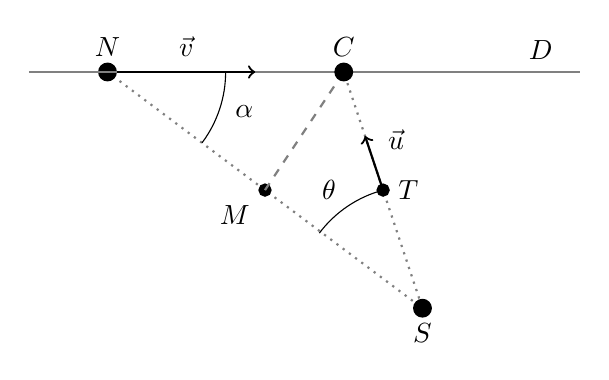
\begin{tikzpicture}
    
    % Le navire
    \node (N) at (-4,0) {};
    \filldraw[black,thick] (N) circle [radius=3pt] ;
    \draw (N) node[above=2pt] {$N$};
    
    % La trajectoire
    \draw[gray, thick] (-5,0) -- (2,0);
    \draw (1.5,0) node[above=1pt] {$D$};
    
    % Le vecteur vitesse
    \node (v) at (-2,0) {};
    \draw[black, thick, ->] (N) -- (v);
    \path (N) -- coordinate[midway](labelv) (v);
    \draw (labelv) node[above=2pt] {$\vec{v}$};
    
    % Le sous marin
    \node (S) at (0,-3) {};
    \filldraw[black,thick] (S) circle [radius=3pt] ;
    \draw (S) node[below=2pt] {$S$};
    
    % La droite
    \draw[gray, thick, dotted] (S) -- (N);
    \draw[black] (-2.5,0) arc (0:-36.9:1.5);
    \draw (-2.5,-0.5) node[anchor=west] {$\alpha$};
    
    % Interception des trajectoires (cible)
    \node (C) at (-1,0) {};
    \filldraw[black,thick] (C) circle [radius=3pt] ;
    \draw (C) node[above=2pt] {$C$};
    
    % Trajectoire de la torpille
    \draw[gray, thick, dotted] (S) -- (C);
    
    % Position de la torpille
    \path (S) -- coordinate[midway](T) (C);
    \filldraw[black,thick] (T) circle [radius=2pt] ;
    \draw (T) node[right=2pt] {$T$};
    
    % Vecter vitesse de la torpille
    \path (T) -- coordinate[midway](u) (C);
    \draw[black, thick, ->] (T) -- (u);
    \path (T) -- coordinate[midway](labelu) (u);
    \draw (labelu) node[above right=1.5pt] {$\vec{u}$};
    
    % angle theta
    \draw[black] (T) arc (105:143:1.5);
    \draw (-1.4,-1.5) node[anchor=west] {$\theta$};
    
    % Projeté orthogonal
    \path (N) -- coordinate[midway](M) (S);
    \filldraw[black,thick] (M) circle [radius=2pt] ;
    \draw (M) node[below left=2pt] {$M$};
    
    \draw[gray, thick, dashed] (M) -- (C);
    
    \end{tikzpicture}
\end{center}
    
    \question Il faut que la trejectoire de la torpille soit minimale : On frappe le navire lorsque il est a la distance minimale. On a alors $\theta = \arctan v/ u$ et $\alpha = \arctan(u / v)$
    
\begin{center}
    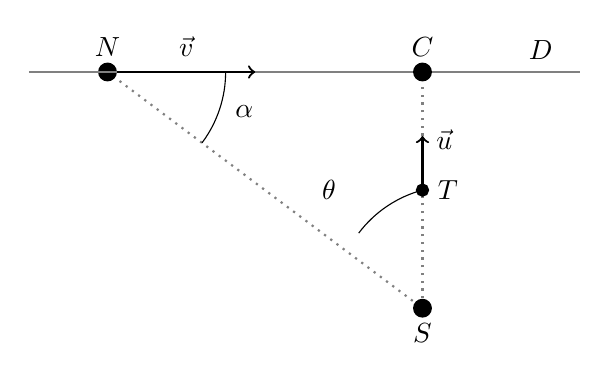
\begin{tikzpicture}
    
    % Le navire
    \node (N) at (-4,0) {};
    \filldraw[black,thick] (N) circle [radius=3pt] ;
    \draw (N) node[above=2pt] {$N$};
    
    % La trajectoire
    \draw[gray, thick] (-5,0) -- (2,0);
    \draw (1.5,0) node[above=1pt] {$D$};
    
    % Le vecteur vitesse
    \node (v) at (-2,0) {};
    \draw[black, thick, ->] (N) -- (v);
    \path (N) -- coordinate[midway](labelv) (v);
    \draw (labelv) node[above=2pt] {$\vec{v}$};
    
    % Le sous marin
    \node (S) at (0,-3) {};
    \filldraw[black,thick] (S) circle [radius=3pt] ;
    \draw (S) node[below=2pt] {$S$};
    
    % La droite
    \draw[gray, thick, dotted] (S) -- (N);
    \draw[black] (-2.5,0) arc (0:-36.9:1.5);
    \draw (-2.5,-0.5) node[anchor=west] {$\alpha$};
    
    % Interception des trajectoires (cible)
    \node (C) at (0,0) {};
    \filldraw[black,thick] (C) circle [radius=3pt] ;
    \draw (C) node[above=2pt] {$C$};
    
    % Trajectoire de la torpille
    \draw[gray, thick, dotted] (S) -- (C);
    
    % Position de la torpille
    \path (S) -- coordinate[midway](T) (C);
    \filldraw[black,thick] (T) circle [radius=2pt] ;
    \draw (T) node[right=2pt] {$T$};
    
    % Vecter vitesse de la torpille
    \path (T) -- coordinate[midway](u) (C);
    \draw[black, thick, ->] (T) -- (u);
    \path (T) -- coordinate[midway](labelu) (u);
    \draw (labelu) node[above right=1.5pt] {$\vec{u}$};
    
    % angle theta
    \draw[black] (T) arc (105:143:1.5);
    \draw (-1.4,-1.5) node[anchor=west] {$\theta$};
    
    
    \end{tikzpicture}
\end{center}
\end{questions}

\end{solution}

\begin{exercise}{Les quatres chiens}{2}{Sup}
{Cinématique}{lelay}

À l'instant $t = 0$, quatre chiens $A$, $B$, $C$ et $D$ initialement situés aux sommets d'un carré de côté $\ell_0$ se mettent en mouvement l'un vers l'autre. $A$ se dirige vers $B$ qui se dirige vers $C$ qui se dirige vers $D$ qui lui-même se dirige vers $A$. Tous les chiens se déplacent à la même vitesse $V$.
\begin{questions}
    \questioncours Donner la définition d'un repère et d'un système de coordonnées. Citer ceux que vous connaissez en expliquant leur fonctionnement.
    \question Faire un schéma. Représenter les positions des chiens ainsi que leurs vecteurs vitesse à $t = 0$, pour $t > 0$ et pour $t = \infty$.
    \question Argumenter que le quadrilatère $ABCD$ reste carré, de côté $\ell(t)$ (on pourra invoquer les symétries de la situation). $\ell(t)$ est-elle une fonction croissante ou décroissante du temps ?
    \question Montrer que $\dv{\ell}{t} = - v$. 
    \question En déduire la durée $t_f$ de la poursuite.
    \question Quelle est la distance $D$ parcourue par chaque chien ?
    \question Déterminer, en coordonnées polaires, l'équation horaire de la trajectoire d'un chien dans un repère à l'origine bien choisie.
\end{questions}

\end{exercise}

\begin{solution}
\begin{questions}
    \questioncours Donner la définition d'un repère et d'un système de coordonnées. Citer ceux que vous connaissez en expliquant leur fonctionnement.
    \question Sa toune
    \question Symétrie SO4, $\ell$ diminue.
    \question Y a plein de manières, On peut écrire $\ell^2 = (\vec{OB} - \vec{OA})^2$, et dériver. 
    \question On a $\dot \ell = - v$ d'où $t_f = \ell_0 / v$, 
    \question Les chiens se déplacent à la vitesse $v$, donc $D = v t_f = \ell_0$
    \question On met le centre au centre. On écrit le vecteur déplacement $\vec{\dd{\ell}}$ de norme $v \dd{t}$ que l'on décompose en deux composantes ($\dd{r}$ sur $\vec{e_r}$ et $r\dd{\theta}$ sur $e_\theta$), d'où $\dot r = \cos \pi/4 v$ et $r\dot\theta = \cos \pi/4 v$ et donc $r(t) = \ell_0 - \frac{\sqrt{2}}{2} vt$ et $\theta(t) =  \int_0^t \frac{\sqrt{2}v}{2r(t)}\dd{t}$
\end{questions}



$t_f = 2/3 \ell_0 / v$, $D = 2 / 3 \ell_0$, en polaire $r = r_0 - \sqrt{3}/2 v t$ et $\theta = V/(2r)$
\end{solution}
,


%%%%%% SUP - DYNAMIQUE (debut)
\setcounter{part}{1} %\part{Mécanique}
\setcounter{section}{3} %\section{Mécanique du point}
% Niveau :      PCSI *
% Discipline :  Méca
% Mots clés :   Ballistique, Mécanique du point, PFD, Chute libre

\begin{exercise}{Parabole de sureté}{2}{Sup, Spé}
{Mécanique,Mécanique du point}{bedo,bermu}

\begin{questions}
\questioncours Conservation de l'énergie mécanique. Cas d'une chute libre.

\uplevel{
On considère un point matériel $m$ en chute libre dans un champ de pesanteur $g$ partant initialement de $(0,0)$ avec une vitesse initiale $$\vv_0 = v_0\cos\theta\ve_x + v_0\sin\theta\ve_z.$$
}

\question Quelle est l'altitude maximale $H$ que $m$ peut atteindre ? Pour quel angle de tir $\theta$ cette altitude est-elle atteinte ?

\question Quelle est la trajectoire $z(x)$ de $m$ ? On exprimera $z$ uniquement en fonction de $x$, $\tan\theta$ et $H$.\\[-2em]
\uplevel{\textbf{\sffamily Indication :} $\dfrac{1}{\cos^2 x} = 1 + \tan^2 x$.

\bigskip

Par la suite, on chercher à tirer sur une cible $M$ de coordonnées $(X,Z)$ avec la balle $m$.

On appelle \emph{parabole de sûreté} la courbe qui enveloppe toutes les trajectoires possibles de $m$, la norme de sa vitesse initiale $v_0$ étant constante.}

\question Déduire de la question précédente l'équation de la parabole de sûreté de ce tir balistique.

\question Qu’en est-il lorsque l’on prend en compte les frottements de l’air ? Donner qualitativement le changement des résultats précédents.
\end{questions}
\end{exercise}

\begin{solution}
\begin{questions}
    \questioncours $\vec{F} = m\vec{a}$
    \question Par intégration : $\vr(t) = -\dfrac{1}{2}\vg t^2 + \vv_0 t$, d'où la parabole
    $$z = -\dfrac{g}{2 {v_0}^2}(1 + \tan^2\theta)x^2 + \tan\theta x.$$
    \question Une considération d'énergie mécanique permet d'obtenir que : $m g h = \dfrac{1}{2}m v_0^2$. L'altitude maximale est donc $h = \dfrac{{v_0}^2}{2g}$, pour $\theta = 0$.
    \question 
    $$z = -\dfrac{1}{4 h}(1 + \tan^2\theta)x^2 + \tan\theta x.$$
     \questionIl faut que
    $$z_0 = -\dfrac{1}{4 h}(1 + \tan^2\theta){x_0}^2 + \tan\theta x_0.$$
    Donc le discriminant par rapport à $\tan\theta$ doit être positif ou nul
    $$h - z_0 - \dfrac{{x_0}^2}{4 h} \geqslant 0.$$
   \questionPour le cas limite on trouve l'équation de la parabole de sûreté
    $$z = h - \dfrac{x^2}{4 h},$$
    telle que si $(x_0,z_0)$ est à l'intérieur, il est touché.
    \question Qualitativement, la parabole de sûreté est plus petite (le projectile va moins haut moins loin), il faut viser plus haut pour aller un peu plus loin (a priori le projectile sera aussi ralenti verticalement dans sa chute que la balle).
\end{questions}
\end{solution}

%\section{Parabole de s\^uret\'e}
%\tags{M\'ecanique du point} \\
%\level{Sup} \\
%\difficulty{1}

%On cherche à tirer un projectile avec une vitesse $V_0$ sur un point $M$. Le but de l'exercice est de trouver un critère simple pour savoir si cela est ou non possible.
%\begin{questions}
%\question \'Ecrire l'\'equation cartésienne $z(x)$ de la parabole décrite par le projectile
%\question Le point $M$ est-il toujours solution de cette équation ?
%\question En déduire l'équation de la parabole de sûreté d'un tir balistique
%\end{questions}

%\section{Tir au pigeon}
%\tags{M\'ecanique du point} \\
%\level{Sup} \\
%\difficulty{2}

%À $t=0$, on tire avec un canon orienté avec un angle $\theta$ sur un objet lâché en chute libre.
%\begin{questions}
%\question On suppose dans un premier temps qu'il n'y a pas de frottements.
%    \begin{parts}
%        \part À quel temps $t$ le projectile atteindra-t-il l'abscisse de la cible ?
%        \part En déduire $\theta$. La puissance du canon est-elle importante ?
%    \end{parts}
%\question On suppose maintenant que le problème prend en compte les frottements.
%    \begin{parts}
%        \part Quels changements attend-t-on par rapport à la situation précédente ?
%        \part Proposer une modélisation des frottements.
%        \part Dans quel cas la situation précédente est-elle toujours vérifiée ?
%    \end{parts}
%\end{questions}

\begin{exercise}{Il touche à tous les coups}{2}{Sup, Spé}
{Mécanique,Mécanique du point}{bedo,bermu}

\begin{questions}
\questioncours Principe fondamental de la dynamique

\uplevel{
On considère un point matériel $P$ en chute libre dans un champ de pesanteur $g$ partant initialement de $(x_0,z_0,0)$ sans vitesse. On cherche à tirer dessus avec une balle $M$ partant de $(0,0)$ avec une vitesse $$\vv_0 = v_0\cos\theta\ve_x + v_0\sin\theta\ve_z.$$
}

\question Quelle est la trajectoire $X(t)$ et $Z(t)$ du point $P$ ?

\question Quelle est la trajectoire $x(t)$ et $z(t)$ de la balle $M$ ?

\question À quel temps $t$ la balle atteindra sa cible ?

\question En déduire la direction $\theta$ qu'il faut viser initialement pour qu’un tir balistique atteigne sa cible si elle est également en chute libre ? En quoi la puissance du canon intervient-elle ? Interpréter ces résultats.
\end{questions}
\end{exercise}
% Niveau :      PCSI
% Discipline :  Méca

\begin{exercise}{Bille sur un cerceau}{2}{Sup}
{Mécanique,Ressort}{lelay}


\begin{questions}
    \questioncours Donner l'énergie potentielle correspondant à un ressort de raideur $k$ et de longueur à vide $\ell_0$.

\begin{EnvUplevel}
On considère une bague pesante de masse $m$ glissant sans frottement sur un cercle de rayon $R$, comme sur le schéma ci-dessous.

\begin{center}
    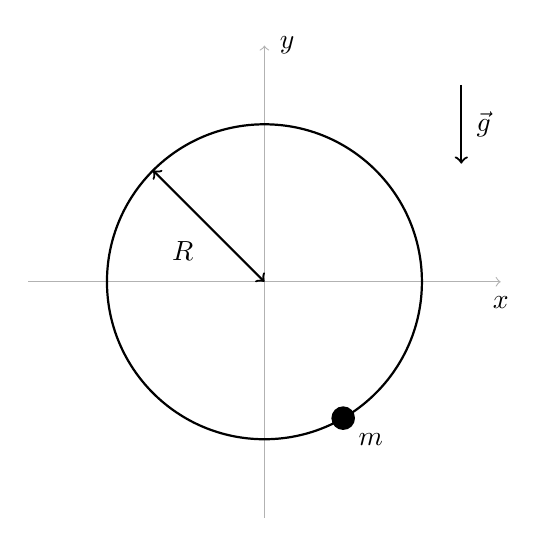
\begin{tikzpicture}
    
    \draw[->, black!30] (-3, 0) -- (3, 0);
    \draw (3,0) node[below=2pt] {$x$};
    
    \draw[->, black!30] (0, -3) -- (0, 3);
    \draw (0,3) node[right=2pt] {$y$};
    
    
    \draw[color=black, thick](0,0) circle (2);
    
    \fill[black] (0.5*2,-0.866*2) circle (0.15);
    \draw (0.5*2,-0.866*2) node[below right=2pt] {$m$};
    
    \draw[<->, thick] (0,0) -- (-0.707*2,0.707*2);
    \draw (-0.707*1,0.707*1) node[below left=2pt] {$R$};
    
    \draw[->, thick] (2.5, 2+0.5) -- (2.5, 2-0.5);
    \draw (2.5,2) node[right=2pt] {$\vec{g}$};
    
    \end{tikzpicture}
\end{center}

\end{EnvUplevel}
    
    \question Donner l'équation du mouvement de la bague. À quel système cette équation vous fait-elle penser ?
    \question En supposant la bille proche du bas du cerceau, quelle approximation permet de linéariser l'équation précédente ? Donner l'équation linéarisée et la famille de solutions correspondante.
    \uplevel{On ajoute maintenant un ressort de raideur $k$ et de longueur à vide $2R$ reliant la bague au point le plus haut du cerceau, comme sur le schéma ci-dessous.}

\begin{center}
    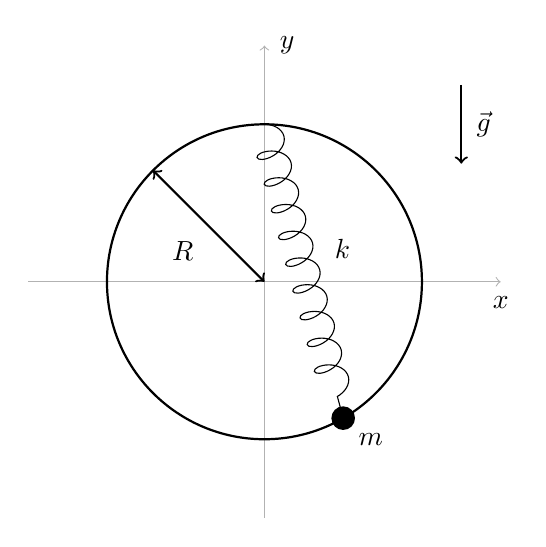
\begin{tikzpicture}
    
    \draw[->, black!30] (-3, 0) -- (3, 0);
    \draw (3,0) node[below=2pt] {$x$};
    
    \draw[->, black!30] (0, -3) -- (0, 3);
    \draw (0,3) node[right=2pt] {$y$};
    
    \draw[color=black, thick](0,0) circle (2);
    
    \fill[black] (0.5*2,-0.866*2) circle (0.15);
    \draw (0.5*2,-0.866*2) node[below right=2pt] {$m$};
    
    \draw[<->, thick] (0,0) -- (-0.707*2,0.707*2);
    \draw (-0.707*1,0.707*1) node[below left=2pt] {$R$};
    
    \draw[->, thick] (2.5, 2+0.5) -- (2.5, 2-0.5);
    \draw (2.5,2) node[right=2pt] {$\vec{g}$};
    
    \draw[decoration={aspect=0.6, segment length=10, amplitude=2mm,coil},decorate] (0,2) -- (0.5*2,-0.866*2);
    \draw (0.7,0.1) node[above right=2pt] {$k$};
    
    \end{tikzpicture}
\end{center}
    \question Donner la nouvelle équation du mouvement de la bague.
    \question En supposant la bille proche du bas du cerceau, développer l'équation jusqu'au premier terme non linéaire. On prendra $k = \frac43 \frac{mg}{R}$.
    \question Quel est l'intérêt de ce dispositif ?

\end{questions}

\end{exercise}

\begin{solution}

\begin{questions}
    \questioncours $E_p = \frac12 k (\ell-\ell_0)^2$
    \question Même dérivation que le pendule (par l'énergie ou la dynamique), on trouve une équation de pendule
    $$ \ddot \theta + {\omega_0}^2\sin \theta = 0$$
    avec $\omega_0 = \sqrt{g / R}$
    \question Équation d'oscillateur harmonique de pulsation $\omega_0$
    \uplevel{On ajoute maintenant un ressort de raideur $k$ et de longueur à vide $\ell_0 = 2R$ reliant la bague au point le plus haut du cerceau, comme sur le schéma ci-dessous.}

    \question 2 possibilités : 
    \begin{itemize}
        \item Rajouter une force de norme $k |\ell - 2R|$. L'angle rajoute un facteur $\sin(\frac\theta2)$.
        
        \item Travailler avec l'énergie mécanique, qui est
    \end{itemize}
    \begin{align*}
    E_m &= E_c + E_{p,g} + E_{p, r} \\
        E_m &= \frac12m R^2\dot{\theta}^2 + mgh + \frac12 k (\ell - 2R)^2
    \end{align*}
    Avec la hauteur $h = - R\cos \theta$ et la longueur du ressort $\ell = 2R \cos(\theta/2)$, d'où
    \begin{align*}
        E_m &= \frac12m R^2\dot{\theta}^2 - mgR\cos\theta + kR (\cos(\theta/2) - 1)^2 \\
        \dd{E_m}/\dd{t} = 0 &= mR^2 \ddot\theta + mgR\sin\theta + 2 kR \sin(\frac{\theta}2)\qty(1 - \cos(\theta/2))
    \end{align*}
    À la fin on doit retomber sur l'équation de la dynamique :
    \begin{align*}
        \ddot{\theta} + \frac{g}{R} \sin\theta + \frac{2k}{m} \sin(\frac{\theta}2)\qty(1 - \cos(\frac{\theta}2)) &= 0
    \end{align*}
    \question À l'ordre 1 le terme supplémentaire ne contribue pas (on a tj un oscillateur harmonique de pulsation $\sqrt{g/L}$). Surprise, les termes d'ordre 3 s'annulent ! Il reste des termes d'ordre 5.
    \question On a réussi à compenser la première non linéarité, on a donc des oscillations plus isochrones

\end{questions}
\end{solution}
% Niveau :      PCSI
% Discipline :  Méca

\begin{exercise}{Balle rebondissante}{2}{Sup}
{Mécanique, Oscillateur harmonique,Ressort}{lelay}

On considère une balle de masse $m$ qui se mouvoir verticalement dans le champ de gravité et sa hauteur par rapport au sol est notée $h$. En dessous de cette balle est accroché un ressort de raideur $k$ et de longueur $\ell_0$. Initialement, la balle est une la hauteur $h_0 > \ell_0$ du sol, et on la laisse tomber à $t = 0$. Attention, le ressort est fixé \textbf{uniquement} à la balle : en particulier, à $t=0$, il ne touche pas le sol.
\begin{questions}
    \questioncours Caractéristiques du mouvement de chute libre : trajectoire, évolution de la position et de la vitesse.
    \question Faire le bilan des forces sur la masse $m$ pour $h > \ell_0$.
    \question Donner les équations du mouvement et leur solution pour $h > \ell_0$
    \question  À quel temps $\tau_1$ la balle arrive-t-elle à une hauteur $\ell_0$ ? Que se passe-t-il alors ? 
    \question Faire le bilan des forces sur la masse $m$ pour $h \leq \ell_0$.
    \question En déduire les équations du mouvement. À quel temps $\tau_2$ la balle revient-elle à une hauteur $\ell_0$ ?
    \question Que se passe-t-il alors ? À quel temps $T$ la balle revient-elle à une hauteur $h_0$ ?
    \question Représenter graphiquement $h(t)$ en identifiant chaque phase du mouvement.
\end{questions}

\begin{solution}

\begin{questions}
    \questioncours Caractéristiques du mouvement de chute libre : trajectoire, évolution de la position et de la vitesse.
    \question C'est une chute libre. $F = -mg$, Le ressort ne touche pas le sol.
    \question $\ddot h = -g$, $\dot h  = -gt$, $h = h_0 - gt^2/2$
    \question À $\tau_1 = \sqrt{2(h_0 - \ell_0)/g}$ le ressort sous la balle touche le sol : le mouvement devient celui d'un système masse-ressort vertical.
    \question $F = -mg - k(h - \ell_0)$. deux forces.
    \question $\ddot h + \frac{k}m h= -g + \frac{k}m \ell_0$. La solution est 
    \begin{align*}
    h (t) &= A\cos(\omega_0t) + B \sin(\omega_0t) + \ell_0 - mg/k \\ 
    h (t) &= A'\cos(\omega_0(t - \tau_1)) + B' \sin(\omega_0(t - \tau_1)) + \ell_0 - mg/k
    \end{align*}
    Avec $\omega_0 = \sqrt{k/m}$. Peu importe le détail des constantes, dans tous les cas le temps mis pour revenir à $\ell_0$ est une période, donc $$\frac{\omega_0}{2\pi} = \frac{1}{2\pi}\sqrt{k/m} $$
    
    % Par ailleurs
    % \begin{align*}
    % h (\tau_1) = A' + \ell_0 - mg/k = \ell_0 \\
    % \dot h (\tau_1) = \omega_0 B' = - g\tau_1
    % \end{align*}
    % D'où $A' = mg/k$ et $B'= -g\tau_1 / \omega_0$
    
    D'où $\tau_2 = \tau_1 + \frac{1}{2\pi}\sqrt{k/m}$
    \question La balle refait une chute libre mais à l'envers, elle met donc encore $\tau_1$ à revenir à $h_0$ ?
    \question Portion de parabole décroissante, portion de sinus, portion de parabole, etc...
\end{questions}
\end{solution}

% VIEILLE VERSION
% On considère un ressort de raideur $k$ et de longueur à vide $\ell_0$ posé verticalement sur une table, sur lequel est posé une masse $m$.
% \begin{questions}
%     \question Déterminer la position d'équilibre notée $z_0$ de la masse $m$ sur l'axe vertical $O_z$ dirigé vers le haut.
%     \question On appuie sur la masse $m$ avec une force $F$ de manière à la déplacer à la position $z_1 < z_0$. Faire le bilan des forces sur la masse $m$ et sur la table.
%     \question À $t=0$, on arrête soudainement d'appuyer sur le système ($F= 0$, $z = z_1$, $\dot{z} = 0$). Appliquer le PFD à la masse $m$ et donner $z(t)$ pour $t>0$.
%     \question Donner la condition pour que le ressort décolle de la table.
%     \question En supposant cette condition vérifiée, trouver l'instant $t_0$ où le ressort décolle. En déduire la vitesse $\dot{z}_0$ de la masse quand elle décolle.
%     \question Donner $z(t)$ pour $t > t_0$. À quelle altitude considérer que le ressort touche de nouveau le sol ?
%     \question Tracer le graphe de $z(t)$ pour $t\in\mbb{R}$ et expliquer chaque étape.
% \end{questions}
\end{exercise}

% Niveau :      PCSI
% Discipline :  Méca

\begin{exercise}{Bifurcation fourche supercritique}{3}{Sup}
{Mécanique,Ressort}{lelay}

On considère une bille de masse $m$ glissant sans frottement sur un rail (l'axe $Ox$) accrochée par un ressort de raideur $k$ et de longueur à vide $\ell_0$ placé à une distance $a$ du rail.
\begin{questions}
    \questioncours Rappeler la définition de point d'équilibre en mécanique
    \question À votre avis, quel va être le mouvement de la bille ? Comment va-t-il évoluer en fonction des paramètres du problème ?
    \question Par la méthode de votre choix, trouver les points d'équilibre de la bille. Combien y en a-t-il ?
    \question Représenter sur un graphe les points d'équilibres (sous forme adimensionnée $u=x_{eq}/a$) en fonction de $r = \ell_0/a$.
    \question On s'intéresse maintenant à la stabilité de ces points d'équilibre. Rappeler comment déterminer la stabilité d'un point d'équilibre. 
    \begin{parts}
        \part On considère le cas $a > \ell_0$. Combien de points d'équilibre y a-t-il ? Quelle est leur stabilité ?
        \part On considère le cas $a < \ell_0$. Combien de points d'équilibre y a-t-il ? Quelle est leur stabilité ?
        \part Redessiner le graphe $u = f(r)$ en prenant compte de la stabilité des points. Pourquoi appelle-t-on cette bifurcation \textit{fourche} supercritique ?
    \end{parts}
    \uplevel{\slshape Vous pouvez choisir de faire les deux prochaines question dans l'ordre que vous souhaitez.}
    \question\textsf{Le noeud du problème (\emph{Calculatoire})}.
    \begin{parts}
        \part Dans le cas où $\ell_0 = a$, combien y-a-t-il de points d'équilibre ? Sans calcul, ce point d'équilibre est-il stable ? 
        \part Écrire le PFD au premier ordre non nul en $x$ près du point d'équilibre. Connaissez vous une solution à cette équation différentielle ?
        \part Tracer le portrait de phase correspondant à cette équation, en déduire que le point d'équilibre est stable. \\
        \textbf{Rappel :} le portrait de phase d'un système est le graphique représentant la vitesse en fonction de la position pour différentes conditions initiales.
        \part En supposant que initialement on a $x = x_0$ et $\dot x = 0$, exprimer la période des oscillations en fonction des paramètres du problème et de l'intégrale
        \begin{align*}
        I &= \int_{-1}^1\frac{dy}{\sqrt{1-y^4}} \approx 2.62
        \end{align*}
        \part Proposer des valeurs pour $m$, $k$, $a$ et $x_0$ et calculer $T$.
    \end{parts}
    \question\textsf{La théorie des catastrophes.}
    \begin{parts}
        \part On suppose maintenant que le rail est incliné d'un angle $\alpha$ par rapport à l'horizontale. Montrer que l'équation que vérifient les points fixes donne sous forme adimensionnée :
        \begin{align*}
            1+\frac{h}u = \frac{r}{\sqrt{1+u^2}}
        \end{align*}
        où $h$ est une constante à déterminer.
        \part En supposant $u \ll 1$, montrer que cette équation se réduit à $u^3+h = (r-1)u$. En prenant $h \ll 1$, dessiner les graphes des fonctions $u \mapsto u^3+h$ et $u\mapsto (r-1)u$ pour $r > 1$ et $r<1$. 
        \part En déduire l'allure du graphe $u = f(r)$. Qu'est ce qui a changé par rapport à la situation précédente ? 
        \part Pour un $r>1$ donné, représenter l'allure de $u = f(h)$. Pouvez-vous expliquer pourquoi cette bifurcation est \textit{catastrophique} ?
    \end{parts}

\end{questions}
 \plusloin La théorie des bifurcations est une étape importante pour l'étude des objets complexes, par exemple les systèmes physiques modélisés par des équations non linéaires.
    
% \begin{figure}{H}
%     \centering
%     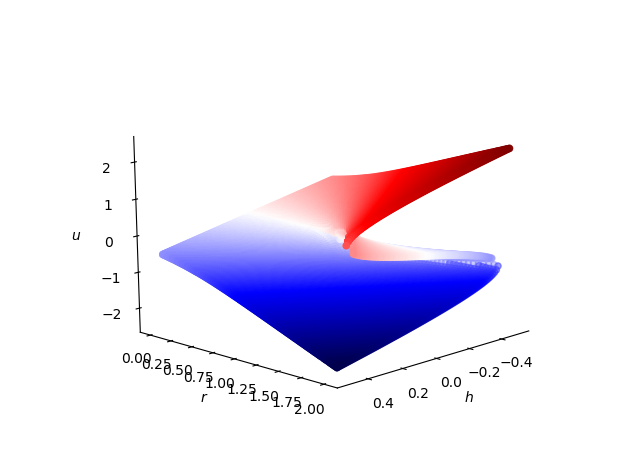
\includegraphics[height=15em]{meca/mecapoint/fourchevraie.png}
%     \caption{Vision pas d'artiste d'une bifurcation fourche supercritique.}
% \end{figure}

% \begin{figure}{H}
%     \centering
%     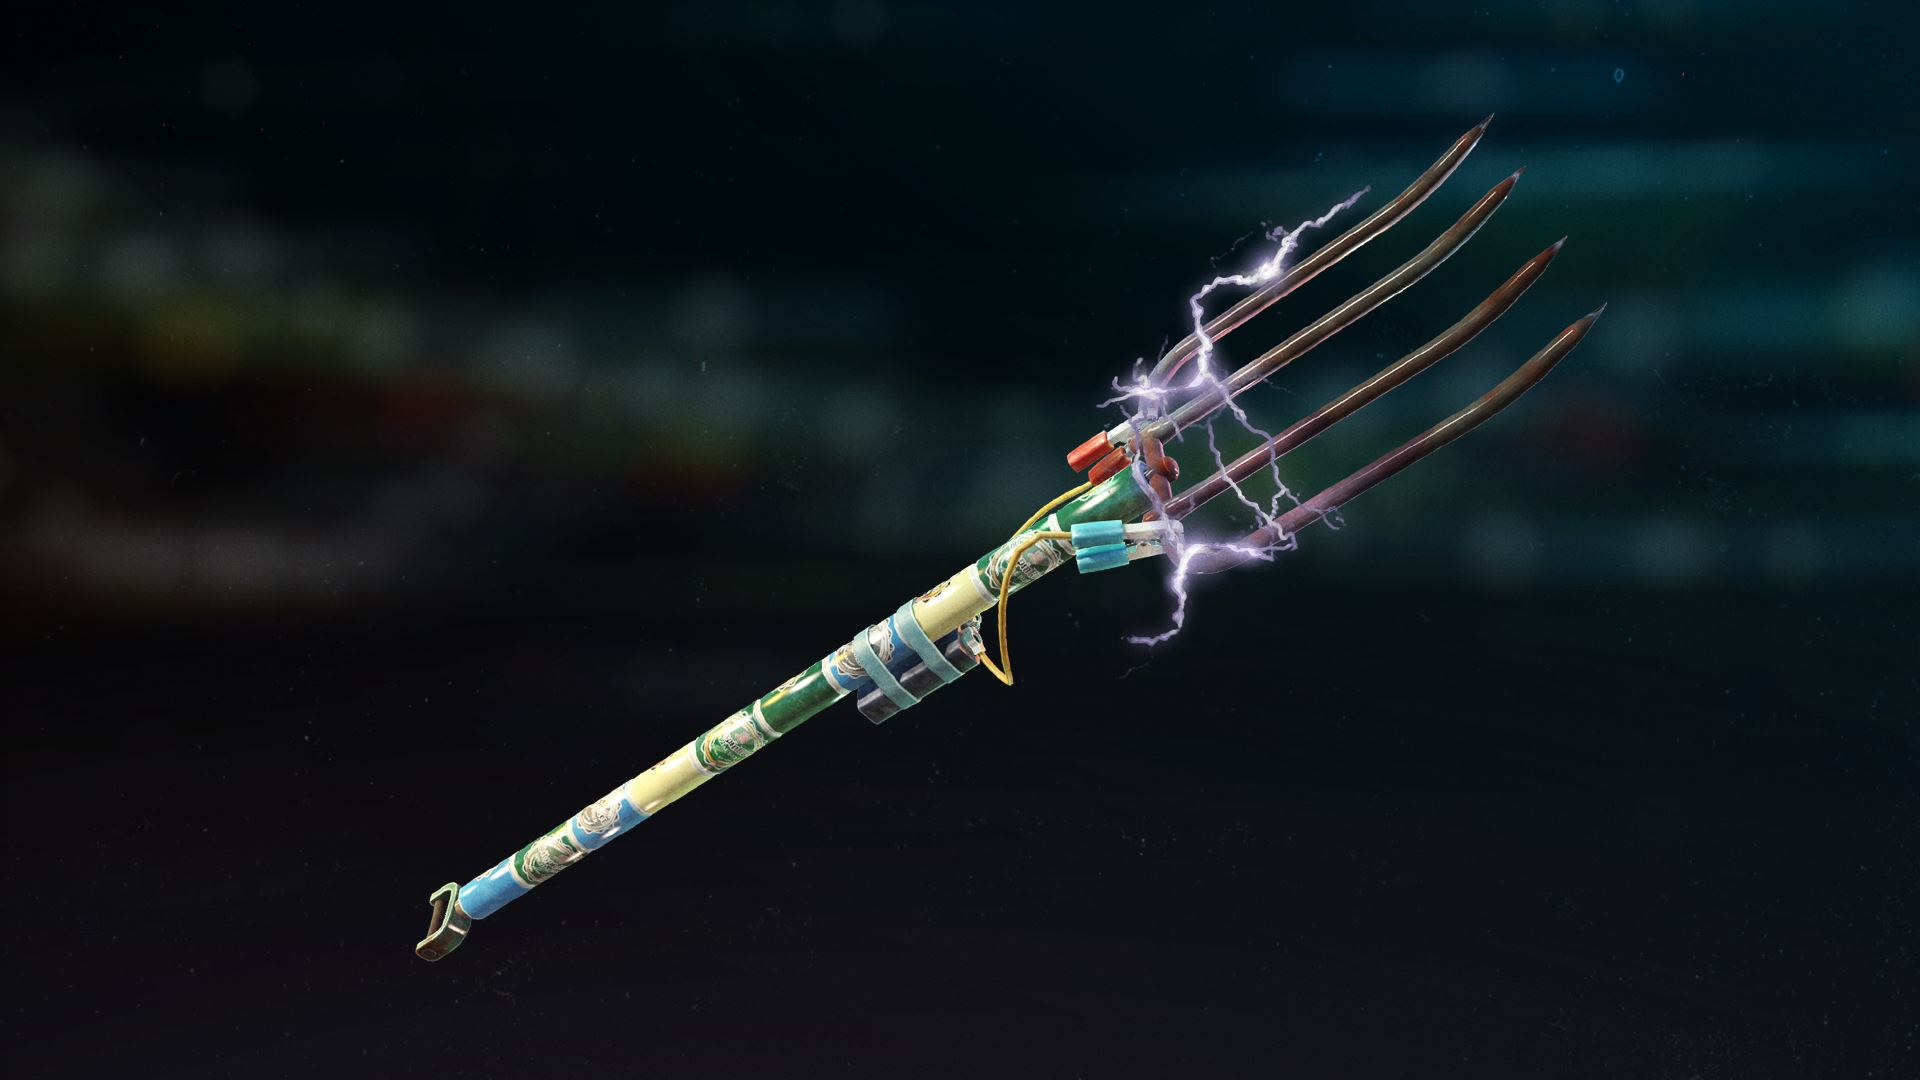
\includegraphics[height=15em]{meca/mecapoint/fourchesupercritique.jpg}%non ! siii ! %gros vilain !
%     \caption{Vision d'artiste d'une fourche supercritique.}
% \end{figure}

\end{exercise}


\setcounter{part}{8} %\part{Chimie}
\setcounter{section}{3} %\section{Cinétique}

\begin{exercise}{Dissociation du dibrome}{1}{PCSI}
{cinetique}{lelay}

Le dibrome Br$_2$ a tendance à se dissocier en deux molécules de brome Br selon la réaction

$$ \text{Br}_2 \longrightarrow 2\, \text{Br} $$

Qui suit une cinétique d'ordre 1 en Br$_2$.

\begin{questions}

    \question Donner l'expression de la concentration en dibrome au cours du temps.
    
\end{questions}
\end{exercise}

\begin{solution}
\begin{questions}

    \question La loi est d'ordre 1, d'où
    $$ v = - \dv{\qty[\text{Br}_2]}{t} = k \qty[\text{Br}_2]$$
    d'où
    $$ \qty[\text{Br}_2](t) = \qty[\text{Br}_2]_0 e^{-kt}$$
    
\end{questions}
\end{solution}

%%%%%%%%%%%%%%%%%%%%%%%%%%%%%%%%%%%%%%%%%%%%%%%%%%%%%%%%%%%%%%%%%%%%%%%%%%%%%%%%%%%%%%%%%%%%%%%%%%%%%%%%%%%%%%

\begin{exercise}{Détemination de l'âge d'une roche}{1}{PCSI}
{cinetique}{lelay}

Lors de sa formation, une roche contenait initialement $7.22\cdot 10^{18}$~noyaux de potassium~40, un isotope du potassium de demie vie $\tau_{1/2} = 1.25\cdot 10^9$~ans.

Aujourd'hui, la même roche ne contient plus que $7.60\cdot 10^{17}$~noyaux de potassium~40.

\begin{questions}

    \question Déterminer l'âge de cette roche
    
\end{questions}
\end{exercise}

\begin{solution}
\begin{questions}

    \question Le nombre de noyaux radioactifs décroit exponentiellement (cinétique d'ordre 1)
    $$ N(t) = N_0 e^{-\lambda t}$$
    avec $\lambda = \ln 2 / \tau_{1/2} = 5.55\cdot 10^{9}$~ans ; d'où
    $$ t = -\frac1\lambda \ln\qty(\frac{N(t)}{N_0}) = 4.06 \time 10^9\text{ ans}$$
    donc 4 milliards d'année.
    
\end{questions}
\end{solution}

%%%%%%%%%%%%%%%%%%%%%%%%%%%%%%%%%%%%%%%%%%%%%%%%%%%%%%%%%%%%%%%%%%%%%%%%%%%%%%%%%%%%%%%%%%%%%%%%%%%%%%%%%%%%%%

\begin{exercise}{Décomposition du bromure de nitrosyle}{1}{PCSI}
{cinetique}{lelay}

Le bromure de nitrosyle se décompose selon la réaction suivante :
$$
\text{NOBr}_\text{(g)} = \text{NO}_\text{(g)} + \frac12\, {\text{Br}_2}_\text{(g)}.
$$
La concentration en bromure de nitrosyle a été mesuré à différentes dates :
\begin{table}[H]
    \centering
    \begin{tabular}{l|c|c|c|c|c|c}
        Temps $t$ (min)             &  0    & 6.2   & 10.8    & 14.7  & 20    & 24.6   \\
        \hline
        Concentration $c$ (mol/L)   & 0.0250    & 0.0191  & 0.0162    & 0.0144    & 0.0125    & 0.0112
    \end{tabular}
    % \caption{Caption}
    % \label{tab:my_label}
\end{table}

\begin{questions}

    \question Déterminer par la méthode intégrale l'ordre de la réaction
    
\end{questions}
\end{exercise}

\begin{solution}
\begin{questions}

    \question Il faut tracer $c = f(t)$ (ordre 0), $\ln c = f(t)$ (ordre 1) et $1/c = f(t)$ (ordre 2) et faire des régressions linéaires.
    
    On trouve des coefficients $r^2$ respectivement de 0.94089, 0.98482 et 0.99999 donc la réaction est d'ordre 2
    
\end{questions}
\end{solution}

%%%%%%%%%%%%%%%%%%%%%%%%%%%%%%%%%%%%%%%%%%%%%%%%%%%%%%%%%%%%%%%%%%%%%%%%%%%%%%%%%%%%%%%%%%%%%%%%%%%%%%%%%%%%%%

\begin{exercise}{Dégradation de l'eau oxygénée}{1}{PCSI}
{cinetique}{lelay}

Une solution d'eau oxygénée contient du peroxyde d'hydrogène H$_2$O$_2$, un produit que se décompose au cours du temps selon la réaction
$$
\text{H}_2\text{O}_2 \longrightarrow \text{H}_2 \text{O} + \frac12\, \text{O}_2
$$
qui suit une loi de vitesse d'ordre 1.

La constante cinétique $k_\text{obs}$ de cette reáction a été mesurée à différentes températures. Les résultats sont présentés dans le tableau ci dessous

\begin{table}[H]
    \centering
    \begin{tabular}{c|c}
        Température & $k_\text{obs}$ (heures$^{-1}$) \\
        20 $^o$C &  0.0065 \\
        30 $^o$C &  0.0144 \\
        40 $^o$C &  0.0276 
    \end{tabular}
    % \caption{Caption}
    % \label{tab:my_label}
\end{table}

\begin{questions}

    \question En utilisant la loi d'Arrhenius, déterminer l'énergie d'activation de la décomposition de l'eau oxygénée. 
    
\end{questions}
\end{exercise}

\begin{solution}
\begin{questions}

    \question Il faut partir de $$k_\text{obs} = A e^{-E_a/RT}$$ pour écrire
    $$
    \ln k_\text{obs} = \ln A - \frac{E_a}{R} \frac{1}{T}
    $$ et faire une régression linéaire en $\ln k_\text{obs}$ et $1/T$.
    
    On trouve $A = 1.7 \cdot 10^7$ h$^{-1}$ et $E_a = 53$~kJ/mol.
    
\end{questions}
Les données sont extraites du mémoire d'Émilie Savage, IMPACT DE LA TEMPÉRATURE SUR LA DÉGRADATION DU PEROXYDE D’HYDROGÈNE LORS DE LA RÉHABILITATION IN SITU D’AQUIFÈRES CONTAMINÉS.
\end{solution}


\setcounter{part}{1} %\part{Mécanique}
\setcounter{section}{3} %\section{Mécanique du point}
% Niveau :      PCSI
% Discipline :  Méca


\begin{exercise}{Dynamique portuaire à Ploudalmézeau}{2}{Sup}
{Oscillateur harmonique}{lelay}

On considère le port breton de Ploudalmézeau dans le Finistère (29). Les principaux habitants en sont de fiers marins bretons, des goélands et des sardines dont les goélands sont friands.

On note $s(t)$ le nombre de sardines et $g(t)$ le nombre de goélands dans le port. Il y a en permanence de nouvelles sardines qui arrivent dans le port, attirées par le charme naturel des côtes bretonnes. De plus les goélands ont tendance à migrer vers l'intérieur des terres et à ne pas rester dans les environs du port. On modélise la situation comme suit :
\begin{align*}
    \dv{g}{t} &= b\:s(t) - \alpha \\
    \dv{s}{t} &= -c\:g(t) + \beta 
\end{align*}
\begin{questions}
    \question Justifier chacun des termes de la modélisation ci-dessus.
    \question Montrer que $g(t)$ et $s(t)$ obéissent chacun à une équation d'oscillateur harmonique de même pulsation.
    \question Trouver $g(t)$ et $s(t)$ sachant que à $t = 0$ jour, il y a 7 goélands et 250 sardines.
    \question Quel est le déphasage entre $g(t)$ et $s(t)$ ? Justifier qu'elles ne peuvent pas être en phase.
\end{questions}
\textbf{Données :} On pourra supposer que à l'équilibre la population de sardines est de 250 individus et celle de goélands de 5 individus, que chaque goéland mange 10 sardines par jour et qu'un nouveau goéland migre vers l'intérieur des terres chaque jour. 
\end{exercise}
% Niveau :      PCSI *
% Discipline :  Méca
% Mots clés :   Ballistique, Mécanique du point, PFD, Chute libre

\begin{exercise}{Le bûcheron canadien}{2}{Sup, Spé}
{Mécanique,Moment cinétique}{bermu}

Un bûcheron canadien veut abattre un pin qui est légèrement incliné suite à une tempête. On assimile cet arbre à une tige longue et homogène de longueur $L$ et de masse $m$. Alors qu'il scie l'arbre à la base du tronc, l'arbre se met à tomber s'appuyant sur la base de la souche, supposée fixe lors de la chute.

On appelle $\theta$ l'inclinaison de l'arbre par rapport à la verticale.

\begin{questions}
    \question \'Etablir l'équation du mouvement de l'arbre lors de sa chute.
    \question Montrer que la vitesse de chute de l'arbre peut s'écrire
    $$\dot{\theta} = \dfrac{1}{\tau}\sqrt{\cos\theta_0 - \cos\theta},$$
    $\tau$ étant un temps caractéristique dont on déterminera l'expression.
    \question En déduire le temps de chute de cet arbre à l'aide de $\tau$ et de la fonction
    $$I(\theta_0) = \int_{\theta_0}^{\pi/2}\dfrac{\dd{\theta}}{\sqrt{\cos\theta_0 - \cos\theta}}.$$
    Quel est le temps du chute pour un arbre de 20m initialement incliné à $5^\circ$ ? Le bûcheron aura-t-il le temps de reculer ?
\end{questions}

\plusloin
Que cela changerait-il si le tronc glissait sur le sol lors de sa chute ? S'il tournait sur sa base ?

\paragraph{Données :}
\begin{itemize}
    \item Le moment d'inertie d'un cylindre fin $J = \frac{1}{3}mL^2$,
    \item Graphe de la fonction $I(\theta_0)$ :
        \begin{figure}[H]
            \centering
            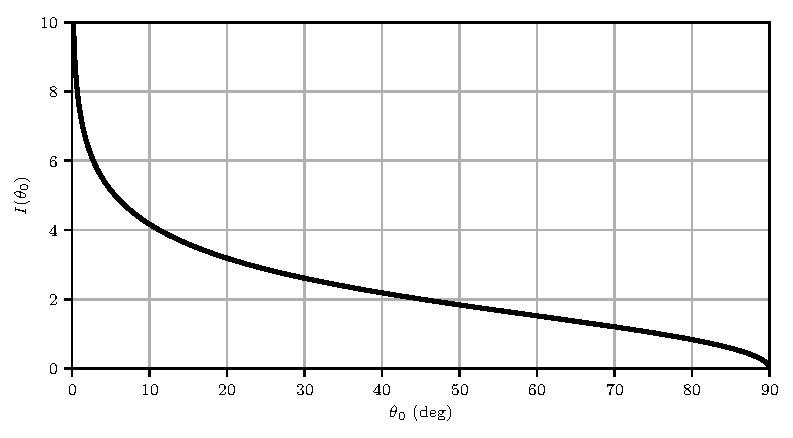
\includegraphics[scale=1]{meca/fonction_I.pdf}
            \vspace{-1em}
            \caption{Graphe de la fonction $I(\theta_0)$.}
        \end{figure}
\end{itemize}

$$\text{En }\theta_0 \rightarrow 0^+, \qquad I(\theta_0) \simeq - \sqrt{2}\ln(\theta_0/\pi).$$
\end{exercise}
% Niveau :      PCSI
% Discipline :  Méca

\begin{exercise}{Balle rebondissante}{2}{Sup}
{Mécanique, Oscillateur harmonique,Ressort}{lelay}

On considère une balle de masse $m$ qui se mouvoir verticalement dans le champ de gravité et sa hauteur par rapport au sol est notée $h$. En dessous de cette balle est accroché un ressort de raideur $k$ et de longueur $\ell_0$. Initialement, la balle est une la hauteur $h_0 > \ell_0$ du sol, et on la laisse tomber à $t = 0$. Attention, le ressort est fixé \textbf{uniquement} à la balle : en particulier, à $t=0$, il ne touche pas le sol.
\begin{questions}
    \questioncours Caractéristiques du mouvement de chute libre : trajectoire, évolution de la position et de la vitesse.
    \question Faire le bilan des forces sur la masse $m$ pour $h > \ell_0$.
    \question Donner les équations du mouvement et leur solution pour $h > \ell_0$
    \question  À quel temps $\tau_1$ la balle arrive-t-elle à une hauteur $\ell_0$ ? Que se passe-t-il alors ? 
    \question Faire le bilan des forces sur la masse $m$ pour $h \leq \ell_0$.
    \question En déduire les équations du mouvement. À quel temps $\tau_2$ la balle revient-elle à une hauteur $\ell_0$ ?
    \question Que se passe-t-il alors ? À quel temps $T$ la balle revient-elle à une hauteur $h_0$ ?
    \question Représenter graphiquement $h(t)$ en identifiant chaque phase du mouvement.
\end{questions}

\begin{solution}

\begin{questions}
    \questioncours Caractéristiques du mouvement de chute libre : trajectoire, évolution de la position et de la vitesse.
    \question C'est une chute libre. $F = -mg$, Le ressort ne touche pas le sol.
    \question $\ddot h = -g$, $\dot h  = -gt$, $h = h_0 - gt^2/2$
    \question À $\tau_1 = \sqrt{2(h_0 - \ell_0)/g}$ le ressort sous la balle touche le sol : le mouvement devient celui d'un système masse-ressort vertical.
    \question $F = -mg - k(h - \ell_0)$. deux forces.
    \question $\ddot h + \frac{k}m h= -g + \frac{k}m \ell_0$. La solution est 
    \begin{align*}
    h (t) &= A\cos(\omega_0t) + B \sin(\omega_0t) + \ell_0 - mg/k \\ 
    h (t) &= A'\cos(\omega_0(t - \tau_1)) + B' \sin(\omega_0(t - \tau_1)) + \ell_0 - mg/k
    \end{align*}
    Avec $\omega_0 = \sqrt{k/m}$. Peu importe le détail des constantes, dans tous les cas le temps mis pour revenir à $\ell_0$ est une période, donc $$\frac{\omega_0}{2\pi} = \frac{1}{2\pi}\sqrt{k/m} $$
    
    % Par ailleurs
    % \begin{align*}
    % h (\tau_1) = A' + \ell_0 - mg/k = \ell_0 \\
    % \dot h (\tau_1) = \omega_0 B' = - g\tau_1
    % \end{align*}
    % D'où $A' = mg/k$ et $B'= -g\tau_1 / \omega_0$
    
    D'où $\tau_2 = \tau_1 + \frac{1}{2\pi}\sqrt{k/m}$
    \question La balle refait une chute libre mais à l'envers, elle met donc encore $\tau_1$ à revenir à $h_0$ ?
    \question Portion de parabole décroissante, portion de sinus, portion de parabole, etc...
\end{questions}
\end{solution}

% VIEILLE VERSION
% On considère un ressort de raideur $k$ et de longueur à vide $\ell_0$ posé verticalement sur une table, sur lequel est posé une masse $m$.
% \begin{questions}
%     \question Déterminer la position d'équilibre notée $z_0$ de la masse $m$ sur l'axe vertical $O_z$ dirigé vers le haut.
%     \question On appuie sur la masse $m$ avec une force $F$ de manière à la déplacer à la position $z_1 < z_0$. Faire le bilan des forces sur la masse $m$ et sur la table.
%     \question À $t=0$, on arrête soudainement d'appuyer sur le système ($F= 0$, $z = z_1$, $\dot{z} = 0$). Appliquer le PFD à la masse $m$ et donner $z(t)$ pour $t>0$.
%     \question Donner la condition pour que le ressort décolle de la table.
%     \question En supposant cette condition vérifiée, trouver l'instant $t_0$ où le ressort décolle. En déduire la vitesse $\dot{z}_0$ de la masse quand elle décolle.
%     \question Donner $z(t)$ pour $t > t_0$. À quelle altitude considérer que le ressort touche de nouveau le sol ?
%     \question Tracer le graphe de $z(t)$ pour $t\in\mbb{R}$ et expliquer chaque étape.
% \end{questions}
\end{exercise}

% Niveau :      PCSI
% Discipline :  Méca

\begin{exercise}{Bille sur un cerceau}{2}{Sup}
{Mécanique,Ressort}{lelay}


\begin{questions}
    \questioncours Donner l'énergie potentielle correspondant à un ressort de raideur $k$ et de longueur à vide $\ell_0$.

\begin{EnvUplevel}
On considère une bague pesante de masse $m$ glissant sans frottement sur un cercle de rayon $R$, comme sur le schéma ci-dessous.

\begin{center}
    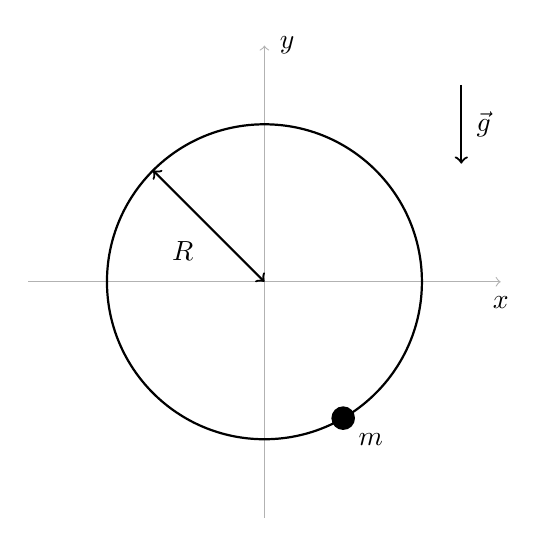
\begin{tikzpicture}
    
    \draw[->, black!30] (-3, 0) -- (3, 0);
    \draw (3,0) node[below=2pt] {$x$};
    
    \draw[->, black!30] (0, -3) -- (0, 3);
    \draw (0,3) node[right=2pt] {$y$};
    
    
    \draw[color=black, thick](0,0) circle (2);
    
    \fill[black] (0.5*2,-0.866*2) circle (0.15);
    \draw (0.5*2,-0.866*2) node[below right=2pt] {$m$};
    
    \draw[<->, thick] (0,0) -- (-0.707*2,0.707*2);
    \draw (-0.707*1,0.707*1) node[below left=2pt] {$R$};
    
    \draw[->, thick] (2.5, 2+0.5) -- (2.5, 2-0.5);
    \draw (2.5,2) node[right=2pt] {$\vec{g}$};
    
    \end{tikzpicture}
\end{center}

\end{EnvUplevel}
    
    \question Donner l'équation du mouvement de la bague. À quel système cette équation vous fait-elle penser ?
    \question En supposant la bille proche du bas du cerceau, quelle approximation permet de linéariser l'équation précédente ? Donner l'équation linéarisée et la famille de solutions correspondante.
    \uplevel{On ajoute maintenant un ressort de raideur $k$ et de longueur à vide $2R$ reliant la bague au point le plus haut du cerceau, comme sur le schéma ci-dessous.}

\begin{center}
    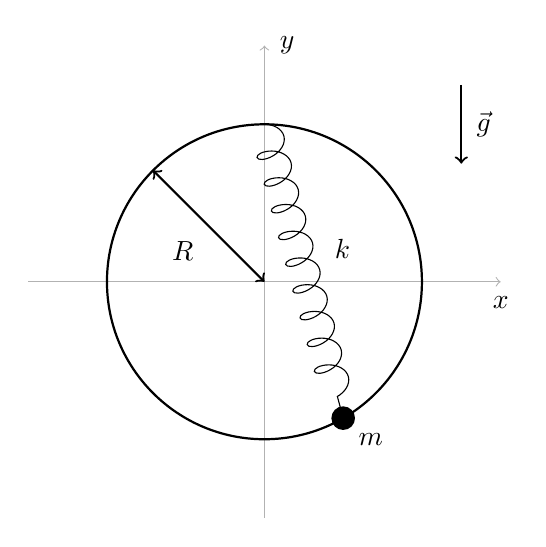
\begin{tikzpicture}
    
    \draw[->, black!30] (-3, 0) -- (3, 0);
    \draw (3,0) node[below=2pt] {$x$};
    
    \draw[->, black!30] (0, -3) -- (0, 3);
    \draw (0,3) node[right=2pt] {$y$};
    
    \draw[color=black, thick](0,0) circle (2);
    
    \fill[black] (0.5*2,-0.866*2) circle (0.15);
    \draw (0.5*2,-0.866*2) node[below right=2pt] {$m$};
    
    \draw[<->, thick] (0,0) -- (-0.707*2,0.707*2);
    \draw (-0.707*1,0.707*1) node[below left=2pt] {$R$};
    
    \draw[->, thick] (2.5, 2+0.5) -- (2.5, 2-0.5);
    \draw (2.5,2) node[right=2pt] {$\vec{g}$};
    
    \draw[decoration={aspect=0.6, segment length=10, amplitude=2mm,coil},decorate] (0,2) -- (0.5*2,-0.866*2);
    \draw (0.7,0.1) node[above right=2pt] {$k$};
    
    \end{tikzpicture}
\end{center}
    \question Donner la nouvelle équation du mouvement de la bague.
    \question En supposant la bille proche du bas du cerceau, développer l'équation jusqu'au premier terme non linéaire. On prendra $k = \frac43 \frac{mg}{R}$.
    \question Quel est l'intérêt de ce dispositif ?

\end{questions}

\end{exercise}

\begin{solution}

\begin{questions}
    \questioncours $E_p = \frac12 k (\ell-\ell_0)^2$
    \question Même dérivation que le pendule (par l'énergie ou la dynamique), on trouve une équation de pendule
    $$ \ddot \theta + {\omega_0}^2\sin \theta = 0$$
    avec $\omega_0 = \sqrt{g / R}$
    \question Équation d'oscillateur harmonique de pulsation $\omega_0$
    \uplevel{On ajoute maintenant un ressort de raideur $k$ et de longueur à vide $\ell_0 = 2R$ reliant la bague au point le plus haut du cerceau, comme sur le schéma ci-dessous.}

    \question 2 possibilités : 
    \begin{itemize}
        \item Rajouter une force de norme $k |\ell - 2R|$. L'angle rajoute un facteur $\sin(\frac\theta2)$.
        
        \item Travailler avec l'énergie mécanique, qui est
    \end{itemize}
    \begin{align*}
    E_m &= E_c + E_{p,g} + E_{p, r} \\
        E_m &= \frac12m R^2\dot{\theta}^2 + mgh + \frac12 k (\ell - 2R)^2
    \end{align*}
    Avec la hauteur $h = - R\cos \theta$ et la longueur du ressort $\ell = 2R \cos(\theta/2)$, d'où
    \begin{align*}
        E_m &= \frac12m R^2\dot{\theta}^2 - mgR\cos\theta + kR (\cos(\theta/2) - 1)^2 \\
        \dd{E_m}/\dd{t} = 0 &= mR^2 \ddot\theta + mgR\sin\theta + 2 kR \sin(\frac{\theta}2)\qty(1 - \cos(\theta/2))
    \end{align*}
    À la fin on doit retomber sur l'équation de la dynamique :
    \begin{align*}
        \ddot{\theta} + \frac{g}{R} \sin\theta + \frac{2k}{m} \sin(\frac{\theta}2)\qty(1 - \cos(\frac{\theta}2)) &= 0
    \end{align*}
    \question À l'ordre 1 le terme supplémentaire ne contribue pas (on a tj un oscillateur harmonique de pulsation $\sqrt{g/L}$). Surprise, les termes d'ordre 3 s'annulent ! Il reste des termes d'ordre 5.
    \question On a réussi à compenser la première non linéarité, on a donc des oscillations plus isochrones

\end{questions}
\end{solution}

\setcounter{part}{4} %\part{Électronique}
\setcounter{section}{2} %\section{Transitoire}
% Niveau :      PCSI - PC
% Discipline :  Elec
% Mots clés :   Elec, Ordre 2

\begin{exercise}{Tube fluorescent}{1}{Sup,Spé}
{\'Electrocinétique, Circuits d'ordre 2}{bermu}


Les tubes fluorescents sont un type particulier de lampes électriques qui produisent de la lumière grâce à une décharge électrique.

Ces tubes s'allument quand la tension à leur bornes dépasse une certaine tension d'allumage $U_a$. Un fois allumé, le tube s'éteint quand la tension descend en dessous de $U_e$, la tension d'extinction, comme l'illustre la figure ci-dessous.

\begin{figure}[H]
    \centering
    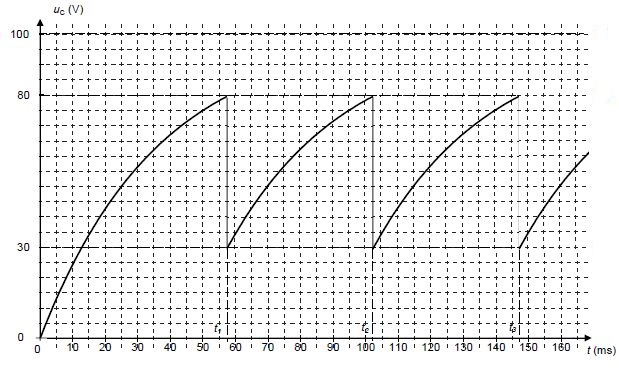
\includegraphics[width=0.65\linewidth]{elec/neon.jpg}
    \caption{Tension au bornes du néon $u_\textsc{c}$ en fonction du temps.}
\end{figure}

\`A $t<0$, le condensateur $C$ est déchargé et le tube est éteint. On allume le générateur à $t=0$.

Le circuit électrique, dans lequel est inséré le tube fluorescent, est schématisé ci-dessous :
\begin{circuit}[Modélisation du tube néon.]
      \draw (0,0)
      to [vsource, v^>=$E$] (0,3)
      to [R, l=$R$] (2,3)
      to [C, l_=$C$, *-*] (2,0)
      to [short] (0,0) {}
      (2,3) to [short] (4,3)
      to [nos, l^=$K$] (4,2)
      to [R, l^=$r$] (4,0)
      to [short] (2,0) {}
      (2.7,0) [open, v_=$u_\textsc{c}$] to (2.7,3) {} ;
      \draw [red, dashed] (3.6,-0.2) rectangle(4.8,3.2) ;
      \node [red] at (4.2,3.5) {Tube néon};
\end{circuit}
Le tube fluorescent est modélisé comme une résistance faible $r$ et un interrupteur $K$ en série. L'interrupteur est ouvert lorsque le tube est éteint et fermé lorsque le tube est allumé.
% Le tube fluorescent est modélisé comme une résistance faible $r$ et un interrupteur $K$ qui s'ouvre et se ferme selon si le tube est allumé ou éteint.

\paragraph{Données :} $E = 100$ V, $R = 60$ k$\Omega$, $r = 10$ $\Omega$, $C = 600$ nF.


\begin{questions}
    \questioncours Condensateurs et dipôles à comportement capacitifs.
    
    \question Décrire le comportement global observé en Fig.~\arabic{exercise}.1 ci-dessus et donner les valeurs de $U_e$ et $U_a$.
    
    \uplevel{On étudie d'abord le circuit entre $t = 0$ et $t_1$.}
    
    \question Simplifier le circuit \arabic{exercise}.1 dans ce cas puis résoudre l'équation différentielle vérifiée par $i$ et $u_\textsc{c}$.
    \question Calculer le temps $t_1$ de l'allumage du néon. Par analogie, quel est le temps $\tau$ du cycle d'allumage du néon ?
    
    \uplevel{On étudie maintenant d'abord le circuit entre $t_1$ et $t_1 + \varepsilon$.}
     
    \question En remarquant que $R\gg r$, simplifier le circuit \arabic{exercise}.1 dans ce cas puis résoudre l'équation différentielle vérifiée par $i$ et $u_\textsc{c}$.
    \question Calculer le temps $t'$ de décharge du condensateur. Justifier que l'on peut négliger ce temps dans le cycle du néon. Voit-on le néon s'allumer et s'éteindre ?
    
\end{questions}
\end{exercise}


\setcounter{part}{8} %\part{Chimie}
\setcounter{section}{2} %\section{Cinétique}
\begin{exercise}{Glycine}{1}{PCSI}
{Acides et bases,Equilibres chimiques}{lelay}

La glycine (ou glycocolle) est un acide aminé de structure H$_2$N--CH$_2$--COOH.  C'est un ampholyte : en effet, dans l'eau, la glycine est engagée dans deux couples acido-basiques de $\text{p}K_\text{a}$ 2.4 et 9.6.

\begin{questions}
    \question Dans l'eau, la glycite est un zwitterion (ou amphion), c'est à dire qu'elle possède à la fois une charge positive et une charge négative. Donner la représentation de Lewis de la glycine dans l'eau.

    \question Écrire les équilibres acido-basiques faisant intervenir la glycine dans l'eau.

    \question Tracer le diagramme de prédominance des espèces de la glycine en fonction du pH de la solution

    \question En solution neutre, quelle est l'espèce majoritaire ?
    
    \question Quel est le pH approché d'une solution de glycine à 10$^{-1}$~M ?
    
    \question L'électrophorèse est une technique permettant de faire migrer les ions d’une solution, sur un support solide, sous l’action d’un champ électrique. À quel pH faut-il opérer l’électrophorèse d’une solution de glycocolle de concentration 10$^{-1}$~M pour que 99\% des ions migrent vers le pôle positif ?
    
\end{questions}
\end{exercise}

\begin{solution}
\begin{questions}

    \question ion glycinium NH$_3^+$ COOH et ion glycinate NH$_2$ COO$^-$
    
    \question ion glycinium - pH 2.4 - glycine - pH 9.6 - ion glycinate
    
    \question À pH = 7 c'est la glycine, l'amphion.
    
    \question On part d'une concentration $C_0 = 0.1$~mol/L en glycine qui réagit selon 2~glycine~=~glycinium~+~glycinate (réaction prépondérante en solution neutre).
    
    On a $K = Ka_2 / Ka_1 = 10^{-7.2}$ c'est bien l'équilibre de contrôle.
    
    Donc d'après le tableau d'avancement [glycinium] = [glycinate] = $x$ et il se trouve que [H$^+$]$^2$ = $Ka_1 \, Ka_2$ d'où $pH = \frac12(pKa_1 + pKa_2) = 6.2$.
    
    \question On veut [glycinate] = 0.99 $c_0$, on ne prend en compte que l'équilibre glycine - glycinate car l'autre est negligeable. 
    
    On utilise la relation de Henderson : $pH = pKa_2 + log([glycinate][glycine]) = 10.6$.
    
\end{questions}
\end{solution}

%%%%%%%%%%%%%%%%%%%%%%%%%%%%%%%%%%%%%%%%%%%%%%%%%%%%%%%%%%%%%%%%%%%%%%%%%%%%%%%%%%%%%%%%%%%%%%%%%%%%%%%%%%%%%%

\begin{exercise}{Imidazole}{1}{PCSI}
{Acides et bases,Equilibres chimiques}{lelay}

L’imidazole, que l’on notera L pour simplifier est une molécule organique de formule C$_3$N$_2$H$_4$. En solution aqueuse, l’imidazole L se comporte comme une monobase faible, le couple LH$^+$/L ayant un $pK_a$ égal à 6.95.

\begin{questions}

    \question On dispose de 50~mL d'une solution acqueuse d'imidazole de concentration 0.02~mol/L. Quel est le pH de cette solution ?

    \question On ajoute à la solution précédente un volume $V$ d’une solution aqueuse d’acide chlorhydrique de concentration 0,50 mol.L$^{-1}$. Calculer, de manière simplifiée, le pH de la solution obtenue correspondant aux valeurs suivantes de $V$ : 0,5 ; 1,0 ; 1,5 ; 2,0 et 2,5 mL.

    \question Représenter l'allure de la courbe $pH = f(V)$
    
\end{questions}
\end{exercise}

\begin{solution}
\begin{questions}

    \question Reaction L = LH+ + HO-, en la supposant peu avancée $K = x^2 / C_0$, on en déduit 
    $$ pH = \frac12\qty( pK_e + pK_a +\log C_0) = 9.6 $$. On a bien pH > pKa + 1 donc L ets majoritaire et pH > 7.5 donc l'autoprotolyse de l'eau est négligeable.
    
    \question La réaction prépondérante est H+ + L = LH+ de constante 10$^{6.95}$ $\gg 1$ donc quantitative.
    \begin{itemize}
        \item Pour V= 0.5, 1.0 et 1.5 mL, on applique juste henderson en supposant que la réaction est totale et pH = 7.4, 6.95, 6.5
        \item Pour V = 2.0 mL tout l'acide a été consommé, la solution est équivalent a une solution d'acide faible LH+ dans 52 mL de solution, d'où $pH = \frac12(pK_a - \log C) = 4.3$
        
        \item Pour V = 2.5 mL on a un excès de 0.25 mmol de H+ pour 52.5 mL de solution. C'est un mélange d'acide faible et d'acide fort. L'acide fort impose le pH d'où $pH = -log [H30+] = 2.3$
    \end{itemize}
    
    \question Typique titrage de baise faible par acide fort.
    
\end{questions}
\end{solution}

%%%%%%%%%%%%%%%%%%%%%%%%%%%%%%%%%%%%%%%%%%%%%%%%%%%%%%%%%%%%%%%%%%%%%%%%%%%%%%%%%%%%%%%%%%%%%%%%%%%%%%%%%%%%%%

\begin{exercise}{Pluies acides}{1}{Sup}
{Acides et bases,Equilibres chimiques}{bermu}

L’eau de pluie est naturellement acide (pH voisin de 6), en raison du dioxyde de carbone qu’elle
dissout. Cette acidification est très nettement augmentée dans les zones à forte activité industrielle. La
pollution par les oxydes de soufre constitue l’une des hypothèses avancées pour expliquer ce
phénomène.

Pour modéliser l’effet de SO$_2$ sur l’acidité de l’eau, on place de l’eau initialement pure dans un récipient
à l’intérieur duquel est maintenue une pression constante de dioxyde de soufre gazeux égale à $\SI{8e-8}{bar}$ à $T = \SI{298}{K}$.

Pour la commodité des calculs, on considère comme négligeable la concentration de SO$_{2\text{(aq)}}$.

\begin{questions}

    \question Tracer le diagramme de prédominance des espèces acido-basiques du soufre intervenant dans la
solution aqueuse.

    \question Sachant que la solution à l’équilibre est plus acide que l’eau de pluie naturelle, quelle espèce du
diagramme de prédominance précédent est assurément en concentration négligeable ?

    \question En déduire l’équation chimique responsable majoritairement de l’acidification de l’eau.

    \question Calculer alors le pH de la solution
    
    \plusloin Vérifier l’hypothèse formulée en \textsfbf{Q2}.
    
\end{questions}

\paragraph{Données :}
$$\text{p}K_\text{a1}(\mathrm{H_2SO_3/HSO_3^-}) = 1,8  \qquad \text{p}K_\text{a2}(\mathrm{HSO_3^-/SO_{3}^{2-}}) = 7,2.$$
Dissolution de SO$_{2\text{(g)}}$ :

$$\mathrm{SO_{2(g)} + H_2O \longrightarrow H_2SO_3} \qquad K_\textsc{h} = \SI{1,25}{}$$

\end{exercise}

\begin{solution}
\begin{questions}

    \question $\mathrm{H_2SO_3/HSO_3^-/SO_{2}}$
    
    \question $\mathrm{SO_{3}^{2-}}$ négligeable

    \question $\mathrm{SO_{2(g)} + 2 H_2O \longrightarrow HSO_3^- + H_3O^+} \qquad K^\circ = K_\textsc{h} 10^{-\text{p}K_\text{a1}} = 0.02$
    
    \question $K^\circ = \dfrac{\mathrm{[H_3O^+][HSO_3^{-}]}}{P_\mathrm{SO_2}}$ or $\mathrm{[H_3O^+] = [HSO_3^{-}] = 10^{-pH}}$

    $\text{pH} = 4.4$.
    
\end{questions}
\end{solution}
\begin{exercise}{Solubilité de l'arséniate de cuivre}{1}{PCSI}
{solubilite,Equilibres chimiques}{lelay}

L'arséniate de cuivre (II) Cu$_3$(AsO$_4$)$_2$ lorsqu'il est plongé dans l'eau libère des ions cuivre (II) Cu$^{2+}$ et des ions arséniates AsO$_4^{3-}$. Sa solubilité dans l'eau pure à 25$^o$C est de 1.74~g.L$^{-1}$. 

\begin{questions}

    \question En déduire sa solubilité molaire et son $pK_s$.
    
    \uplevel{On mélange un volume $V_1 = 10$~mL de solution de sulfate de cuivre (II) à $c_1 = 1.6\cdot10^{-2}$~mol.L$^{-1}$ et un volume $V_2 = 40$~mL de solution d'arséniate de sodium à $c_2 = 2.0\cdot10^{-2}$~mol.L$^{-1}$.}

    \question Observe-t-on l'apparition d'un précipité ?

    \question Même question avec $c_1 = 8.0\cdot 10^{-2}$~mol.L$^{-1}$.
    
\end{questions}
Données : $M(\text{Cu}) = 63.5$~g.mol$^{-1}$, $M(\text{As}) = 75$~g.mol$^{-1}$ et $M(\text{O}) = 16$~g.mol$^{-1}$
\end{exercise}

\begin{solution}
\begin{questions}

    \question Masse molaire totale 468.5 g/mol d'où solubilité molaire 3.71~mmol/L
    
    $n$ moles dans un litre d'eau pure donnent $3s$ moles de Cu$^{2+}$ et $2s$ moles de AsO$_4^{3-}$ d'où $K_s = (3s)^3(2s)^2  =108 s^5$ avec $s = 3.71$~mmol/L d'où $K_s = 7.59\cdot 10^{-11}$ et $pK_s = -\log K_s = 10.1$
    
    \question Concentration en cuivre : $3.2$~mmol/L ; en ions arséniates $16$~mmol/L ; quotient réactionnel $Q = 8.4\time 10^{-12}$.
    
    $Q < K_s$ \textbf{donc il n'y a pas précipitation}
    
    \question Concentration en cuivre : $16$~mmol/L ; quotient réactionnel $Q = 1.0\time 10^{-9}$.
    
    $Q > K_s$ \textbf{donc il y a précipitation}
    
\end{questions}
\end{solution}

\begin{exercise}{Effet d'ion commun}{1}{PCSI}
{solubilite,Equilibres chimiques}{lelay}

Le chlorure d'argent est un solide dont la solubilité dans l'eau pure est de 1.92~mg/L.

\begin{questions}

    \question En déduire sa solubilité molaire et son $pK_s$.
    
    \uplevel{On verse maintenant du chlorure d'argent non pas dans l'eau pure mais dans une solution de chlorure de potassium de concentration $c$.}

    \question Sans calculs, que dire de la solubilité du chlorure d'argent dans ce cas ?

    \question Trouve la solubilité du chlorure d'argent pour $c = 10$~mmol/L.
    
\end{questions}
Données : $M(\text{Ag}) = 107.87$~g.mol$^{-1}$, $M(\text{Cl}) = 35.45$~g.mol$^{-1}$
\end{exercise}

\begin{solution}
\begin{questions}

    \question Masse molaire totale 143.32 g/mol d'où solubilité molaire $1.341\times 10^{-5}$~mol/L
    
    $n$ moles dans un litre d'eau pure donnent $s$ moles de Ag$^{+}$ et $s$ moles de Cl${-}$ d'où $K_s = s^2$ avec $s = 1.341\times 10^{-5}$~mol/L d'où $pK_s = -\log K_s = 9.752$
    
    \question Il y a déjà du chlore ionique dans la solution, la solubilité sera donc moindre.
    
    \question On a cette fois $Ks = s (c + s)$. Si on est malin on voit que nécessairement $s \ll c$, sinon il faut résoudre une équation du second degré. À la fin, $s = 1.8\times 10^{-8}$ mol/L
    
\end{questions}
\end{solution}

\begin{exercise}{Mélange d'halogénure d'argent}{1}{PCSI}
{solubilite,Equilibres chimiques}{lelay}

On dispose dans un bécher d’un volume $V_0 = 100$~mL d’une solution aqueuse de chlorure de sodium $C_1 = 100$~mmol/L et de bromure de sodium $C_2 = 200$~mmol/L. Les deux composés sont supposés parfaitement dissous. On dispose d’autre part d’une solution de nitrate d’argent de concentration $C = 1.00$~mol/L dans une burette de 50 mL.

\begin{questions}

    \question Tracer les domaines d'existence des précipités AgCl et AgBr en fonction de $p\text{Ag}$ ($p\text{Ag}=10^{-[Ag^+]/C^0}$)
    
    \uplevel{On introduit maintenant progressivement le nitrate d'argent de la burette dans le becher.}

    \question Sans calculs, que va-t-il se passer ? Peut-on récupérer un précipité absolument pur ? Lequel ?

    \question Quel est la quantité maximale théorique de ce précipité pur qu'il est possible de récupérer ? Calculer le rendement de cette opération.
    
\end{questions}
Données : $pK_s(\text{AgCl}) = 9.8$, $pK_s(\text{AgBr}) = 12.3$.
\end{exercise}

\begin{solution}
\begin{questions}

    \question Masse molaire totale 143.32 g/mol d'où solubilité molaire $1.341\times 10^{-5}$~mol/L
    
    $n$ moles dans un litre d'eau pure donnent $s$ moles de Ag$^{+}$ et $s$ moles de Cl${-}$ d'où $K_s = s^2$ avec $s = 1.341\times 10^{-5}$~mol/L d'où $pK_s = -\log K_s = 9.752$
    
    \question Quand $p\text{Ag}$ diminue, càd quand $[\text{Ag}^+]$ augmente, AgBr se forme, puis AgCl à partir du moment où $p\text{Ag}$ passe en dessous de 8.8. On peut donc obtenir AgBr pur.
    
    \question Le cas limite correspond à arrêter de verser lorsque $p\text{Ag} = 8.8$ i.e. $[Ag^+] = 10^{-8.8}$ M. 

    On a alors $[Br^-] = \frac{K_s}{[Ag^+]} = 10^{-3.5}$ M.

    Soit $V$ le volume versé et $n$ la quantité de solide formée. Alors on a 
    \begin{align*}
        C_2 V_0 &= [Br](V_0 + V) + n \\
        C V &= [Ag](V_0 + V) + n \\
    \end{align*}
    On en déduit $V(C+[Br]-[Ag]) = V_0(C_2 + [Ag]-[Br])$. Puisque $[Ag], [Br] \ll C_2, C$ alors $V\approx V_0 C_2/C = 20$~mL.
    D'où $n = C_2 V_0 - [Br] (V_0+V) = 0.200*0.1 - 10^{-3.5} (0.1 + 0.02) = 19.96$ mmol. Au début on en avait 20.0, d'où un rendement de 99.8 \%.
\end{questions}
\end{solution}

\setcounter{part}{5} %\part{Electromag}
\setcounter{section}{2} %\section{Electrostat}
\input{electromag/electrostat/brevesgauss}
% Niveau :      PC
% Discipline :  Electromagnétisme
%Mots clés :    Equations de Maxwell, Debye-Hückel

\begin{exercise}{Cerceau -- Dipole}{3}{Spé}
{\'Electromagnétisme,\'Electrostatique,Statique des fluides}{bermu}

\begin{questions}
    \questioncours Quelle est l'expression du potentiel $V(\vr)$ et du champ $\vE(\vr)$ électriques de deux charges ponctuelles de signes opposés $\pm q$ distantes de $d$. \\
    Sans calcul, comment généraliser cela à une distribution continue ?
\begin{EnvUplevel}

On considère une distribution linéaire de charge électrique de forme circulaire, de rayon $R$ et de charge totale $q$. On appelle $O$ le centre du cercle. 

On définit $Oz = (O, \ve_z)$ l'axe de symétrie de la distribution. On étudiera uniquement les effets de la distribution pour une charge test située en $Oz$.
\end{EnvUplevel}
    \question Faire un schéma de la situation et introduire un système de coordonnées pertinent.
    \question Discuter les éléments de symétrie de la distribution et en déduire la forme attendue du champ $\vE(z)$ pour un observateur situé sur $Oz$.
    \question Calculer la contribution au potentiel électrique $\dd{V}(z)$ d'un élément $\dd{q}$ de la distribution --- qu'on exprimera dans le système de coordonnées choisi --- pour un observateur situé en $z$ sur $Oz$.
    \question En déduire le potentiel total $V(z)$ généré par le cercle en $z$, puis le champ électrique $\vE(z)$.
    \question Soit une charge test $q'$ contrainte sur l'axe $Oz$. Etablir la dynamique de $q'$ proche de $z = 0$.
\uplevel{On considère que cette charge $q' = -q$ est désormais fixée en $z = d$.}
    \question Quel est le potentiel total $V'$ ressenti pour un observateur en $z$ ?
    \question Montrez que la distribution totale se comporte comme un dipôle, dont on calculera le moment dipolaire $\vec{p}$.
    \question Quid du cas $d = 0$ ?
\end{questions}


\end{exercise}

\begin{solution}
\begin{questions}
    \questioncours 
    \question
    \question
    \question $\dd{V} = \dfrac{q\dd{\theta}/2\pi}{4\pi\varepsilon_0 \sqrt{R^2 + z^2}}$
    \question $V = \dfrac{q}{4\pi\varepsilon_0 \sqrt{R^2 + z^2}}$, $\vE = \dfrac{q z}{4\pi\varepsilon_0 (R^2 + z^2)^{3/2}}$
\end{questions}
\end{solution}

\setcounter{part}{5} %\part{Electromag}
\setcounter{section}{3} %\section{Magnétostat}
\begin{exercise}{Piège de Ioffe--Pritchard}{2}{Spé}
{Magnétostatique}{bermu, lelay}

\paragraph{Point méthode en électromagnétisme :}
\begin{itemize}
    \item à partir de la géométrie de problème, choisir le bon système de coordonnées ;
    \item utiliser les invariances du problème pour réduire le nombre de variables ;
    \item utiliser les symétries pour réduire le nombre de composantes ;
    \item identifier une surface fermée, un contour \emph{etc.} et appliquer le théorème intégral pertinent.
\end{itemize}


\begin{questions}
    \questioncours Exprimer le champ magnétique $\vB(\vr)$ d'un cylindre de rayon $R$ parcouru par un courant $I$, réparti volumiquement. On présentera les résultats d'électromagnétisme utiles.
    \question Justifier rapidement que l'on puisse écrire $\vB(\vr) = \rot(A(r)\ve_z)$, et trouver l'expression de $A(r)$ pour le champ précédent.
    \uplevel{On considère désormais le dispositif suivant : quatre fils conducteurs sont disposés aux sommets d'un carré de côté $2a$ et sont parcourus par des courants $+I$ et $-I$, alternativement.}
    \question Quelle est l'expression du potentiel vecteur $A(x, y)$ en un point $M$ d'un plan $(O, x, y)$ dont l'origine et les axes auront été judicieusement choisis ?
    \question Exprimer $A$ à l'ordre le plus bas pour $x$ et $y$ proches de l'origine.
    \question En déduire le champ magnétique $\vec{B}$ pour un point proche de l'origine. Son expression est-elle cohérente avec les invariances et les symétries de cette nouvelle configuration ? 
    \uplevel{On place dans ce champ un neutron de moment magnétique $\vec{m}$. À l'aide de techniques de pompage optique, il est possible de maintenir le moment magnétique du neutron dans la direction opposée de celle du champ.}
    
    \question Par analogie avec un dipôle électrique, donner l'énergie magnétique $E_m$ d'un tel neutron placé dans un champ $\vB$.
    
    \question Tracer la courbe $E_m(\rho)$ avec $\rho = \sqrt{x^2+y^2}$ pour le système étudié et commenter l'appellation "piège" de Ioffe pour ce dispositif.
    % \question On place dans ce champ un neutron de moment magnétique $\vec{m}$. Justifiez que le moment magnétique du neutron s'aligne avec celui du champ magnétique.
    % \question Quelle est la force appliquée par le champ magnétique sur le neutron ? En déduire la dynamique du neutron. Commenter l'appellation "piège" de Ioffe pour ce dispositif.
\end{questions}

\paragraph{Données :} 
% Rotationnel en coordonées cartésiennes
% $$\rot\vA = \qty(\pdv{A_z}{y} - \pdv{A_y}{z}) \ve_x
% + \qty(\pdv{A_x}{z} - \pdv{A_z}{x}) \ve_y
% + \qty(\pdv{A_y}{x} - \pdv{A_x}{y}) \ve_z$$ 
Rotationnel en coordonnées cylindrique
$$\rot\vA = \qty(\dfrac{1}{r}\pdv{A_z}{\theta} - \pdv{A_\theta}{z}) \ve_r
+ \qty(\pdv{A_r}{z} - \pdv{A_z}{r}) \ve_\theta
+ \qty(\dfrac{1}{r}\pdv{}{r} (r A_\theta) - \dfrac{1}{r}\pdv{A_r}{\theta}) \ve_z$$ 

\end{exercise}

\begin{solution}

\begin{questions}
    \questioncours $\vB(\vr) = \mu_o I/2\pi r \ve_\theta$
    \question On a $\vB(\vr) = \rot(A(r)\ve_z) = -\pdv{A}{r}\ve_\theta$ soit ici $A(r) = \mu_0 \frac{I}{2\pi}\ln(\frac{r}{R})$
    \uplevel{On considère désormais le dispositif suivant : quatre fils conducteurs sont disposés aux sommets d'un carré de côté $2a$ et sont parcourus par des courants $+I$ et $-I$, alternativement.}
    \question Les axes passent par les fils et le centre est au centre, les quatre distances aux fils sont $r_1 = \sqrt{x^2 + (a+y)^2}$, $r_2 = \sqrt{(a+x)^2 + y^2}$, $r_3 = \sqrt{x^2 + (a-y)^2}$, $r_4 = \sqrt{(a-x)^2 + y^2}$ et on a $$ A(x,y) =  \mu_0 \frac{I}{2\pi}\qty( \ln(\frac{r_1}{R}) - \ln(\frac{r_2}{R}) + \ln(\frac{r_3}{R}) - \ln(\frac{r_4}{R}) ) $$
    \question Attention il faut garder les termes d'ordre 2 c'est un peu degueulasse.
    \begin{align*}
        r_{1,3} & = a\sqrt{1 \pm 2\frac{y}{a} + \frac{x^2}{a^2} + \frac{y^2}{a^2}} \\
        &\approx a\qty(1 + \frac12\qty(\pm 2\frac{y}{a} + \frac{x^2}{a^2} + \frac{y^2}{a^2}) - \frac18\qty(2\frac{y}{a})^2) \\
        & = a\qty(1 \pm \frac{y}{a} + \frac12\frac{x^2}{a^2}) \\
        \ln(r_{1,3}) &= \ln\frac{a}{R} + \ln(1 \pm \frac{y}{a} + \frac12\frac{x^2}{a^2}) \\
        &\approx \ln\frac{a}{R} \pm \frac{y}{a} + \frac12\frac{x^2}{a^2} - \frac12\qty(\frac{y}{a})^2 \\
        &= \ln\frac{a}{R} \pm \frac{y}{a} + \frac12\frac{x^2-y^2}{a^2}
    \end{align*}
    et ainsi $r_{2,4}$ en échangeant $x$ par $y$ et vice versa.
    
    D'où
    \begin{align*}
        A(x,y) &=  \mu_0 \frac{I}{2\pi} \bigg(&& \\
        & &&+      \ln\frac{a}{R} + \frac{y}{a} + \frac12\frac{x^2-y^2}{a^2}\\ 
        & &&- \qty(\ln\frac{a}{R} + \frac{x}{a} - \frac12\frac{y^2-x^2}{a^2}) \\
        & &&+      \ln\frac{a}{R} - \frac{y}{a} + \frac12\frac{x^2-y^2}{a^2} \\
        & &&- \qty(\ln\frac{a}{R} - \frac{x}{a} + \frac12\frac{y^2-x^2}{a^2}) \\
        & &&\bigg)\\
        &=  \mu_0 \frac{I}{2\pi}\bigg(&& 2\frac{x^2-y^2}{a^2} \bigg) 
    \end{align*}
    
    \question On a $A(r) = \mu_0 \frac{I}{\pi}\frac{x^2-y^2}{a^2} $ et $B = (\partial_y A , -\partial_x A , 0) = -\mu_0 \frac{2I}{\pi a^2}(y, x, 0)$, $B$ ne dépend toujours pas de $z$.
    \uplevel{On place dans ce champ un neutron de moment magnétique $\vec{m}$. À l'aide de techniques de pompage optiques utilisant des faisceaux laser, il est possible de maintenir le moment magnétique du neutron dans la direction opposée de celle du champ.}
    
    \question $E_m = -\vec{m}\cdot \vB = m \abs{B}$ dans le cas où ils sont antiparallèle.
    
    \question On a $\abs{B} \propto \sqrt{x^2 +y^2}$ d'où $Em \propto \rho$ : on a bien un piège.
\end{questions}
\end{solution}

\begin{exercise}{Piège de Penning}{2}{Spé}
{Magnétostatique}{lelay}

On souhaite réaliser un champ électrostatique permettant de confiner des particules de charge $q > 0$ et de masse $m$ au voisinage d'un point $O$ dans le vide.

\begin{questions}
    \questioncours Équation de Maxwell--Gauss, équation de Poisson pour le potentiel.
    \uplevel{On envisage dans un premier temps de réaliser ce confinement en créant un champ électrostatique approprié. On admet qu'il est toujours possible de choisir un système d'axes $(Oxyz)$ pour que le développement limité du potentiel près de $O$ puisse s'écrire}
    $$
    V(x, y, z) = V_0 + a_1 x + a_2 y + a_3 z + b_1 x^2+ b_2y^2 + b_3z^2 + \order{\abs{\vr}^2}
    $$
    \question Comment doivent être les coefficients $b_i$ pour que le point $O$ soit un point d'équilibre ? Quid des $a_i$ et de $V_0$ ?
    \question Quelle équation locale est vérifiée par le potentiel, et qu'implique-t-elle quant aux coefficients $b_i$ ? Montrer qu'en conséquence de l'équation de Maxwell-Gauss, il est impossible de confiner une charge au voisinage d'un point en utilisant le seul champ électrique.
    \uplevel{On suppose qu'un arrive à réaliser à l'aide du système d'électrodes approprié le champ électrique $\vec{E}$ dérivant du potentiel $V$ si dessous}
    $$
    V(x, y, z) = -\frac{E_0}{2d}(x^2+y^2-2z^2)
    $$
    \question Une particule chargée positivement soumise à ce potentiel est confinée sur le plan $z = 0$. En déduire le signe de $E_0$. Qu'en est-il du mouvement de la particule dans le plan $xy$ ?
    \question On ajoute à l'installation un dispositif générant un champ $\vec{B} = B_0 \ve_z$ (Bonus : comment réaliser un tel champ expérimentalement ?). Établir l'équation différentielle vérifiée par $u = x+  iy$.
    \question Montrer que si le champ magnétique dépasse une valeur critique $B_c$, il est possible de confiner la particule.
    \question Déterminer $x(t)$ et $y(t)$ pour $B_0 \gg B_c$ en prenant comme condition initiale $\vec{OM} = x_0 \ve_x$ et $\vec{v}(0) = \vec{0}$. On fera apparaître deux pulsations caractéristiques.
    
\end{questions}

\paragraph{Données :} 
% Rotationnel en coordonées cartésiennes
% $$\rot\vA = \qty(\pdv{A_z}{y} - \pdv{A_y}{z}) \ve_x
% + \qty(\pdv{A_x}{z} - \pdv{A_z}{x}) \ve_y
% + \qty(\pdv{A_y}{x} - \pdv{A_x}{y}) \ve_z$$ 
Rotationnel en coordonnées cylindriques
$$\rot\vA = \qty(\dfrac{1}{r}\pdv{A_z}{\theta} - \pdv{A_\theta}{z}) \ve_r
+ \qty(\pdv{A_r}{z} - \pdv{A_z}{r}) \ve_\theta
+ \qty(\dfrac{1}{r}\pdv{}{r} (r A_\theta) - \dfrac{1}{r}\pdv{A_r}{\theta}) \ve_z$$ 

\end{exercise}

\begin{solution}
\begin{questions}
    \questioncours --
    \uplevel{On envisage dans un premier temps de réaliser ce confinement en créant un champ électrostatique approprié. On admet qu'il est toujours possible de choisir un système d'axes $(Oxyz)$ pour que le développement limité du potentiel près de $O$ puisse s'écrire}
    $$
    V(x, y, z) = V_0 + a_1 x + a_2 y + a_3 z + b_1 x^2+ b_2y^2 + b_3z^2 + \order{\abs{\vr}^2}
    $$
    \question Les $b_i$ doivent être positifs (Il faut un minimum global de potentiel), les $a_i$ doivent être nuls (0 est le minimum, pas un autre point) et $V_0$ peut importe, invariance de jauge le potentiel est défini à une constante près.
    \question Équation de Poisson, $\triangle V = 0$ donc au moins un des $b_i$ est positif : on ne peut pas faire de piège électrostatique.
    \uplevel{On suppose qu'un arrive à réaliser à l'aide du système d'électrodes approprié le champ électrique $\vec{E}$ dérivant du potentiel $V$ si dessous}
    $$
    V(x, y, z) = \frac{E_0}{2d}(x^2+y^2-2z^2)
    $$
    \question On a le long de l'axe $z$ $F_z = -eE_0 \frac{z}{d}$, qui est une force de rappel élastique ssi  $E_0 > 0$. Par contre en $z=0$ (dans le plan $xy$) on a $F_{xy} = qE = e -\grad_{xy} V = eE_0 \frac{x+y}{2d}$ : ça diverge exponentiellement !
    \question On a $$ \ddot u - i \omega_B \dot u - \frac{1}{\tau^2}u = 0 $$
    avec $\omega_B = \frac{qB}{m}$ la pulsation cyclotron et $\tau = \sqrt{md/q E_0}$ le temps typique d'éloignement de la particule.
    \question Le déterminant de l'équation caractéristique est $(-i\omega_b)^2 - 4(-1/\tau^2) = 4/\tau^2 - \omega_B^2$ qui est négatif (racine imaginaires pures, solutions purement oscillantes donc système stable) pour $\omega_B > 2/\tau$ soit $B_0 > 2\sqrt{E_0 m/ dq}$
    \question Les pulsations d'oscillations sont 
    \begin{align*}
        \omega_\pm &= \frac{\omega_B}{2}\qty(1 + \sqrt{1 - \frac{1}{\tau^2\omega_B^2}}) \\
        &\approx \omega_B \qqtext{ou bien} 1/2\tau^2\omega_B
    \end{align*} 
    soit une pulsation ra[ide et une pulsation lente.
    
\end{questions}
\end{solution}


\begin{exercise}{Vitesse d'un satellite sur son orbite elliptique}{2}{Sup}
{Mécanique, Moment cinétique}{correge}

On considère un satellite de masse 1 tonne en orbite elliptique autour de la Terre. Le satellite se maintient sur cette trajectoire car il est soumis à la force gravitationnelle qu’exerce sur lui la Terre. Cette force est en permanence dirigée vers le centre de la Terre. On note :
\begin{itemize}
    \item $O$ le centre de la Terre qui est un des foyers de l’ellipse;
    \item $C$ le centre de l’ellipse;
    \item $A$ l’apogée du satellite (point de l’orbite le plus éloignée de la surface de la Terre);
    \item $P$ son périgée (point de l’orbite le plus proche de la surface de la Terre);
    \item $A'$ le point de la surface de la Terre qui fait face à A, l’apogée du satellite;
    \item $P'$ le point de la surface de la Terre qui fait face à P, le périgée du satellite;
    \item $S$ le point tel que $\vec{CS}$, vertical dirigé vers le haut, représente le demi-petit axe de l’ellipse.
\end{itemize}
On donne les grandeurs suivantes :
\begin{itemize}
    \item Distance $CS=16715$km;
    \item Distance $AA'=35000$km;
    \item Distance $PP'=350$km;
    \item Distance $OA'=OP'=RT=6400$km;
\end{itemize}
On considère que le satellite est en mouvement dans un référentiel galiléen dont le centre est situé au centre de la Terre.

\begin{questions}
    \questioncours Moment cinétique.
    \question Réaliser une figure comportant toutes les indications de l’énoncé. Représenter le satellite en $S$ avec sa vitesse $\vec v$ et les vecteurs polaires unitaires.
    \question La vitesse en $S$ est $v_S=\SI{14650}{km.h^{-1}}$. Calculer le moment cinétique du satellite en $S $ par rapport au point $O$ (un angle permettant de repérer le satellite peut être utile).
    \question En appliquant le théorème du moment cinétique, trouver la vitesse du satellite à son apogée $A$ et à son périgée $P$.
\end{questions}

\end{exercise}

\begin{solution}
\begin{questions}
    \questioncours 
    \question 
    \question $L_O(S)=mvCS=\SI{2.4e17}{kg.m^2.s^{-1}}$
    \question Avec le théorème du moment cinétique, on trouve un moment cinétique est constant. On sait qu'au périgée et à l'apogée, rayon vecteur et vitesse sont orthogonales. Donc $v_A=\SI{5.9e3}{km.h^{-1}}$, $v_P=\SI{3.6e4}{km.h^{-1}}$
\end{questions}

\end{solution}


\begin{exercise}{Pendule simple incliné}{2}{Sup}
{Mécanique, Moment cinétique}{correge}

On réalise un pendule simple à l’aide d’un mobile autoporteur sur table à coussin d’air. Le mobile de masse $m$ est accroché à l’extrémité d’un fil de longueur $\ell$ dont l’autre extrémité est attachée à un point fixe $O$ de la table.Le mobile peut alors se déplacer sans frottement dans un plan $xOy$.

\begin{center}
    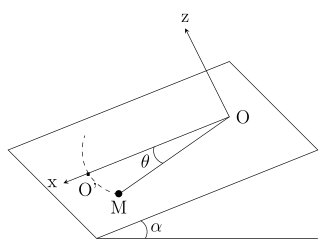
\includegraphics[scale=0.6]{meca/mecasolides/pendule_incline}
\end{center}

\begin{questions}
    \questioncours Moment cinétique.
    \question Exprimer le moment cinétique de $M$ par rapport à $O$.
    \question Identifier les forces et exprimer leur projection sur la base cylindrique.
    \question Appliquer le théorème du moment cinétique afin d’établir l’équation différentielle du mouvement dans le cas des petites oscillations.
    \question En déduire l’expression de la période des petites oscillations.
    \question Le pendule est lancé depuis sa position d’équilibre $O$’ avec un vitesse initiale $v_0$. Quel est l’angle maximal atteint (l’hypothèse des petites oscillations étant toujours valable) ?
\end{questions}

\end{exercise}

\begin{solution}
\begin{questions}
    \questioncours 
    \question $L = m\ell^2 \dot{\theta}^2$
    \question $\vec{P} = mg(\sin \alpha \cos \theta, -\sin \alpha \sin \theta,  -\cos \alpha)_{(r,\theta,z)}$
    \question $\ddot \theta + \theta \frac{g}{\ell}\sin \alpha = 0$
    \question $\omega_0^2 = \frac{g}{\ell}\sin \alpha$
    \question On trouve la solution, et on cherche le maximum. On trouve $\theta_{max} = \frac{v_0}{\ell \omega_0}$
\end{questions}

\end{solution}


\begin{exercise}{Usine alimentée par un courant sinusoïdal}{1}{Sup}{\'Electrocinétique,Régime sinusoidal forcé}{correge}

\begin{questions}
    \questioncours Montrer le lien entre valeur efficace et amplitude pour un signal sinusoïdal.

    \uplevel{Une usine, alimentée sous la tension sinusoïdale de valeur efficace $U=\SI{220}{V}$ et de fréquence $f=\SI{50}{Hz}$, consomme une puissance moyenne $P=\SI{100}{kW}$; son facteur de puissance est $\cos \phi=0.8$.}
    
    \question Calculer l'intensité efficace $I$. \\ On pourra montrer que $P$ ne dépend que de $U$ et $I$ et $\cos\phi$, $\phi$ étant le déphasage entre $u(t)$ et $i(t)$.

    \uplevel{Souvent, les installations industrielles et domestriques ont un caractère inductif (\emph{i.e.} se comportent comme une inductance résistive), lié à la présence de fils et de bobinages (moteurs, transformateurs~\emph{etc.}).}

    \question Représenter qualitativement dans le plan complexe $\ubar{u}$ et $\ubar{i}$ en prenant comme référence la phase de $\ubar{u}$, ainsi que l'argument $\varphi$ de l'impédance équivalente $\ubar{Z}$ de l'usine.

    \question EDF facture à l'usine la puissance moyenne consommée $P$. Sachant que le réseau pour acheminer l'électricité possède une résistance $R_\textsc{edf}$, quelle puissance $P_\text{f}$ doit fournir EDF en fonction de $P$, $R_\textsc{edf}$ et $I$ ? Que doit valoir $\phi$ pour réduire la charge sur le réseau ?
    
    \uplevel{EDF met en parallèle avec l'usine un condensateur de capacité $C$ de sorte que le facteur de puissance $\cos\phi_\text{tot}$ de l'ensemble soit maximal.}

    \question Compléter la figure de la question 3 en y représentant les amplitudes complexes de $\ubar{i}_C$ et $\ubar{i}_\text{tot}$.

    \question Que doit valoir $C$ pour que le facteur de puissance $\cos\phi = 1$ ? Calculer en pourcentage l'économie réalisée par le fournisseur de l'énergie électrique, l'industriel consommant toujours la même puissance.
\end{questions}
\end{exercise}

\begin{solution}
    \begin{questions}
        \question La valeur efficace est telle que :
        $$U^2 = \ev{u(t)^2} = {u_0}^2 \ev{\cos^2(\omega t)} = \dfrac{1}{2}{u_0}^2 \ev{1 + \cos(2\omega t)} = \dfrac{{u_0}^2}{2}.$$
        D'où $U = u_0/\sqrt{2}$.

        \question $P = \ev{u(t) i(t)} = 2 UI\ev{\cos(\omega t)\cos(\omega t + \phi)} = UI\ev{\cos\phi + \cos(2\omega t + \phi)} = UI\cos\phi$.

        AN. : $I = 568$ A.

        \question $\ubar{u} = \ubar{Z}\, \ubar{i}$, donc $u_0 = Z_0 i_0 e^{j(\phi + \varphi)}$, ce qui indique que $\varphi = -\phi$, l'angle entre $(Ox)$ et $\ubar{i}$. Comme $\ubar{Z} = R + jL\omega$, $0 < \varphi < \pi/2$ et donc $0 > \phi > -\pi/2$, quart bas droite du plan complexe.

        Ainsi $\cos\phi \ll 1$ : on diminue la puissance consommée.

        \question $$P_\text{f} = R_\textsc{edf} I^2 + \abs{Z}\cos\phi I^2 = \dfrac{R_\textsc{edf} I^2 + \abs{Z}\cos\phi}{\cos^2\phi}\dfrac{P^2}{U^2}.$$
        Ainsi pour une même puissance, la charge sur réseau diverge quand $\cos\phi = 0$, EDF tente donc d'optimiser en prenant $\phi = 0$.

        \question $\ubar{i}_C = jC\omega \ubar{u}$ sera donc dans l'axe $Oy$.
        
        $\ubar{i}_\text{tot} = \ubar{i} + \ubar{i}_C = j\qty(C\omega - \dfrac{1}{Z_0}\sin\varphi) + \dfrac{1}{Z_0}\cos\varphi\ubar{u}$ sera entre les deux.

        Pour que $\phi_\text{tot} = 0$, il faut que $\text{Im }\ubar{i}_C = - \text{Im }\ubar{i}$ soit $I_C = I \sin\varphi$ ou encore $C\omega = \dfrac{1}{Z_0}\sin\varphi$.

        \question Ainsi $C = \dfrac{\sin\varphi}{Z_0\omega}$. L'industriel économise donc d'un facteur $\dfrac{1 - \cos\phi}{\cos\phi} = 25\%$.
        
    \end{questions}
\end{solution}

\begin{exercise}{Condensateur plan}{1}{Spé}
{Electromagnetisme, Theoreme de gauss}{lelay,bermudez}

\paragraph{Point méthode en électromagnétisme :}
\begin{itemize}
    \item à partir de la géométrie de problème, choisir le bon système de coordonnées ;
    \item utiliser les invariances du problème pour réduire le nombre de variables ;
    \item utiliser les symétries pour réduire le nombre de composantes ;
    \item identifier une surface fermée, un contour \emph{etc.} et appliquer le théorème intégral pertinent.
\end{itemize}

\begin{questions}
    \questioncours Énoncé du théorème de Gauss. \\
    Donner sa version locale. Comment passe-t-on de l'un à l'autre ?
    \uplevel{On considère un plan infini dans le vide, en $z=0$, uniformément chargé par une charge surfacique~$\sigma$.}
    \question Donner l'expression du champ électrique $\vec{E}$ engendré par le plan chargé, en veillant bien à distinguer plusieurs cas.
    \uplevel{On considère maintenant deux plans infinis et parallèles, l'un de charge surfacique $\sigma$ placé en $z = -d/2$ et l'autre de charge surfacique $-\sigma$ placé en $z = d/2$.}
    \question Quel est le champ électrique résultant hors des deux plans ($\abs{z} > d/2$) ? Quel est le champ électrique entre les deux plans ($\abs{z} < d/2$) ?
    \question Quel est le potentiel électrique $V(z)$ à l'intérieur et à l'extérieur du condensateur.
    \question On appelle $U$ la différence de potentiel entre les deux plans. Exprimer $U$ en fonction de $\sigma$, $d$ et $\epsilon_0$.
    \question Dans un condensateur électrique, quelle est le lien entre sa charge $q$, la différence de potentiel $U$ sa capacité $C$ ? En déduire le lien entre $C$ et les caractéristiques géométriques du condensateur (sa surface $S$, nottament). 
    \uplevel{En réalité, le milieu entre les deux armatures n'est pas le vide mais un diéléctrique (il faut donc remplacer $\ep_0$ par $\ep_0\ep_r$).}
    \question \textsf{Application numérique :} condensateur céramique constitué d'armatures circulaires de diamètre 5 mm et d'une épaisseur de 1 $\mu$m de céramique de permittivité $\ep_r = 200$, $\ep_0 = \SI{8.9e-12}{F.m^{-1}}$.
								  
    %\questionbonus On suppose maintenant que l'espace entre les plaques la distribution suivante de charge volumique dans l'espace : $\rho(x, y, z \geq 0) = \rho_0 e^{-z/\lambda}$ où $\lambda$ est une constante, et $\rho(x, y, z<0) = 0$. Quel est le champ électrique $\vec{E}(x, y, z)$ pour $z < 0$ ? Pour $z \geq 0$ ?
\end{questions}

\end{exercise}


\begin{exercise}{Cylindre infini}{1}{Spé}
{Electromagnetisme, Theoreme de gauss}{lelay,bermudez}

\paragraph{Point méthode en électromagnétisme :}
\begin{itemize}
    \item à partir de la géométrie de problème, choisir le bon système de coordonnées ;
    \item utiliser les invariances du problème pour réduire le nombre de variables ;
    \item utiliser les symétries pour réduire le nombre de composantes ;
    \item identifier une surface fermée, un contour \emph{etc.} et appliquer le théorème intégral pertinent.
\end{itemize}

\begin{questions}
    \questioncours Énoncé du théorème de Gauss. \\
    Donner sa version locale. Comment passe-t-on de l'un à l'autre ?
    \uplevel{On considère un cylindre de rayon $R$ de longueur infinie dans le vide, uniformément chargé par une charge volumique $\rho$.}
    \question Donner l'expression du champ électrique $\vec{E}$ engendré par le cylindre chargé, en veillant bien à distinguer plusieurs cas.
    \question Donner l'expression du potentiel électrique $V(r)$ correspondant. Que se passe-t-il quand $r$ tend vers l'infini ? Est-ce physique ? Quelle hypothèse de départ cause ce problème ?
    %\question On considère maintenant la quantité $u = \frac12 \epsilon_0 \vec{E}^2$, qui a la dimension d'une énergie par unité de volume. Quelle est l'énergie contenue dans un cylindre de rayon $r \leq R$ et de hauteur $H$ ? Même question pour $r \geq R$.
								  
    %\question En remplaçant le cylindre infini par une sphère de rayon $R$, calculez l'énergie contenue dans une sphère de rayon $r \geq R$. Quelle est la limite de cette énergie lorsque $r$ tend vers l'infini ?
\end{questions}

\end{exercise}



\begin{exercise}{La Terre creuse}{1}{Spé}
{Electromagnetisme, Theoreme de gauss}{lelay,bermudez}

\paragraph{Point méthode en électromagnétisme :}
\begin{itemize}
    \item à partir de la géométrie de problème, choisir le bon système de coordonnées ;
    \item utiliser les invariances du problème pour réduire le nombre de variables ;
    \item utiliser les symétries pour réduire le nombre de composantes ;
    \item identifier une surface fermée, un contour \emph{etc.} et appliquer le théorème intégral pertinent.
\end{itemize}

\begin{questions}
    \questioncours Énoncé du théorème de Gauss. \\
    Donner sa version locale. Comment passe-t-on de l'un à l'autre ?
    \uplevel{On considère une sphère de rayon $R_1$ dans le vide, uniformément chargée par une charge volumique $\rho$.}
    \question Donner l'expression du champ électrique $\vec{E}_1$  engendré par la sphère chargée, en veillant bien à distinguer plusieurs cas.
    \question On considère maintenant une autre sphère dans le vide de charge $-\rho$ et de rayon $R_2 < R_1$. Quel est le champ $\vec{E}_2$ généré par cette seconde sphère ?
    \question En déduire le champ engendré une sphère creuse, uniformément chargée par une densité volumique de charge $\rho$ comprise entre les rayons interne $R_2$ et externe $R_1$.
	 
		  
		  
		  
	  
    \question Que penser des théories de la Terre creuse selon lesquelles la Terre est en fait creuse et qu'une partie de l'humanité pourrait habiter à l'intérieur ?
    %\question On considère maintenant une sphère de rayon $R$ et de charge $Q$ et on introduit la quantité $u = \frac12 \epsilon_0 \vec{E}^2$, qui a la dimension d'une énergie par unité de volume. Quelle est l'énergie contenue dans une sphère de rayon $r \leq R$ ? $r \geq R$ ? Dans tout l'espace ?
\end{questions}

\end{exercise}

\begin{exercise}{Foudre dans un pré}{2}{Spé}
{Electrostatique}{correge}

Un éclair frappe le sol au milieu d'un pré, à proximité d'une vache. Nous cherchons à savoir si cette vache est en sécurité. On modélise la foudre par un fil rectiligne vertical semi-infini, parcouru par un courant $I$. La vache se trouve à une distance $d$ du point d'impact, et la distance entre ses pattes est notée $p$. 

\begin{center}
    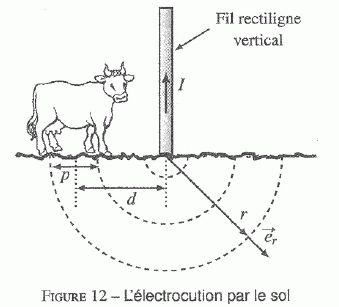
\includegraphics[width=0.4\linewidth]{electromag/electrostat/vache_foudre.png}
\end{center}

\begin{questions}

    \question Déterminer la densité de courant électrique $\vec{j}$ dans le sol.
    \question Rappeler l'expression de la loi d'ohm locale. Exprimer le champ électrique dans le sol et en déduire son potentiel $V(r)$ en le supposant nul à l'infini.
    \question Exprimer en fonction de $p$ et $d$ les potentiels au niveau des pattes avant et arrière de la vache. Quelle est la tension entre les pattes de la vache ?
    \question A quelle distance minimale $d_m$ du point d'impact est-elle en sécurité ?
    
    
    
\end{questions}

\paragraph{Données :} 
\begin{itemize}
    \item Foudre : $I=\SI{15}{kA}$
    \item Conductivité électrique du sol : $\gamma = \SI{1}{S/m}$
    \item Résistance de la vache : $R= \SI{30}{k\Omega}$
    \item Distance entre les pattes : $p=\SI{1.5}{m}$
    \item Courant létal pour une vache : $I_{max} = \SI{25}{mA}$
\end{itemize}

\end{exercise}

\begin{solution}
\begin{questions}

    \question $\vec j(r) = \frac{-I}{2\pi r^2} \vec{e}_r$
    \question $V(r) = \frac{-I}{2\pi \gamma  r} $
    \question $U = V(d+\frac{p}{2}) - V(d+\frac{p}{2}) \approx \frac{Ip}{2\pi \gamma d^2} $
    \question $d_m = \sqrt{\frac{Ip}{2\pi \gamma R I_{max} }}$
    
\end{questions}
\end{solution}


% Niveau :      sup
% Discipline :  Méca

\begin{exercise}{Fluctuation de la durée du jour}{3}{Sup, spé}
{Mécanique,Moment cinétique}{bermudez}


\begin{questions}
    \questioncours Présenter l'analogie entre moment cinétique et quantité de mouvement, et discuter de leur conservation. On fera un tableau pour comparer les différentes grandeurs en jeu dans chaque cas.
    \uplevel{
La durée du jour, $\tau_\text{j}$, actuellement de 24h, fluctue sur des échelles de temps très variées allant de quelques jours sur plusieurs millions d'années. La figure ci-dessous représente la variation de la durée d'une journée depuis les années 1900.

\begin{figure}[H]
    \centering
    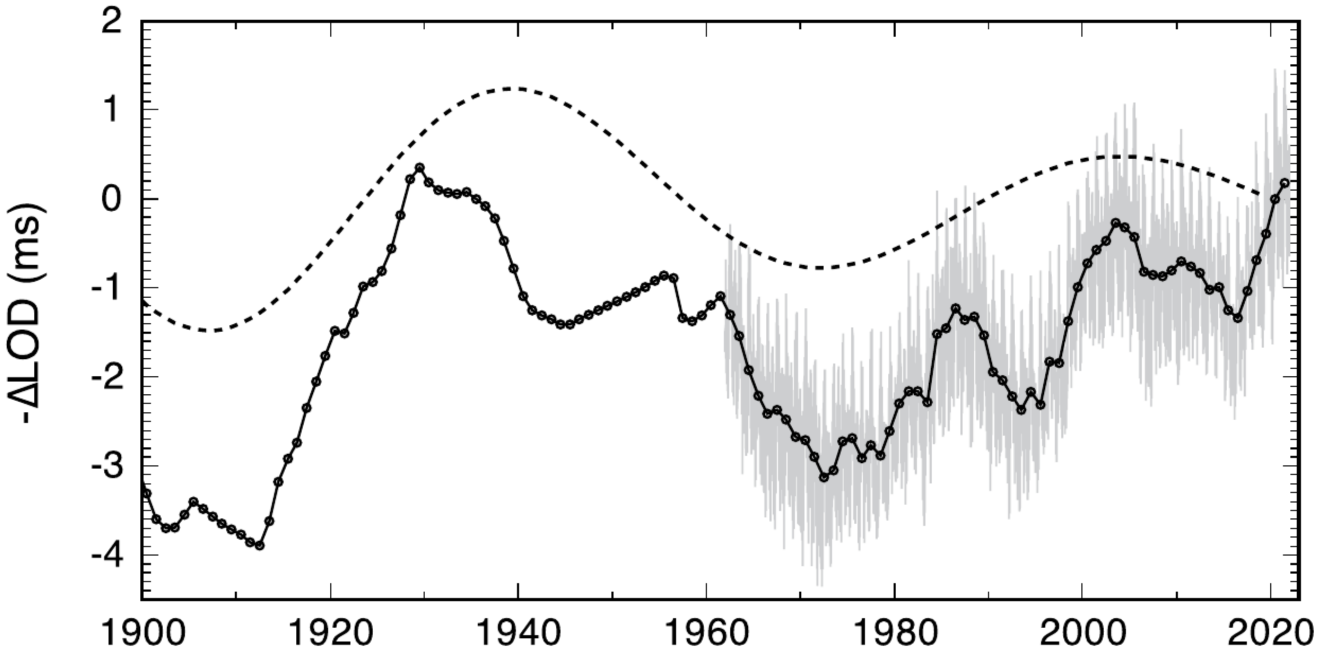
\includegraphics[width=.7\linewidth]{meca/mecasolides/lengthoftheday.png}
    \caption{Variation de la durée d'une journée en millisecondes par rapport aux 24h standard.}
    \label{fig:LOD}
\end{figure}

Il y a plusieurs million d'années, elle était de 22h. Par l'effet du couplage Terre--Lune, elle a augmentée graduellement avec le temps.

Il a été mis en évidence très récemment, que la durée du jour pouvait également fluctuer sur des périodes d'environ 70 ans (en pontillés sur la figure~\ref{fig:LOD}) à cause du renversement de la rotation du noyau interne de la Terre, qui libre de tourner dans le noyau externe, liquide, est presque immobile depuis 2013.

La durée du jour fluctue également sur des échelles de temps plus courtes par couplage entre l'atmosphère et la Terre. Pour des échelles de temps de l'ordre de quelques jours à quelques années (en gris sur la figure~\ref{fig:LOD}), cela est principalement attribué aux courants atmosphériques globaux, comme les alizés (vents d'est, à l'équateur en basse altitude), les vents d'ouest (latitude $30^\circ$, basse altitude) et les jet stream (vents d'ouest aux latitudes $60^\circ$ en haute altitude), qui ont des vitesses qui varient sur des valeurs de l'ordre de 100 km/h typiquement.

\textsf{Problème ouvert :} en utilisant les résultats de la question précédente et à l'aide des données, estimer en ordre de grandeur les quantités suivantes :
}

    \question la fluctuation d'une journée due à l'arrêt de la rotation du noyau interne de la Terre ;
    \question la fluctuation d'une journée due aux courants atmosphériques globaux ;
    \question l'éloignement moyen entre la Terre et la Lune en cm/siècle.
\end{questions}

\paragraph{Données :}(toutes ne sont pas utiles)\\[-2em]
\begin{multicols}{2}
\begin{itemize}
    \item masse de la Terre : $m_\textsc{t} = 6,0\times 10^{24}$ kg ;
    \item masse de la Lune : $m_\textsc{l} = 7,4\times 10^{22}$ kg ;
    \item masse de l'atmosphère : $m_\text{a} = 5,3\times 10^{18}$ kg ;
    \item densité normale de l'air au niveau de la mer : $\rho = 1,3\ \mathrm{kg\cdot m^{-3}}$ ;
    \item densité myenne du noyau interne : $\rho = \SI{12 300}{kg/m3}$ ;
    \item distance Terre--Lune : 384 400 km ;
    \item rayon moyen de la Terre : $R_\textsc{t} = 6371$~km ; 
    \item rayon moyen du noyau interne : $R_\text{n} = 1220$~km ;
    \item constante universelle de gravitation : $G = 6,67\times 10^{-11}$ SI ;
    \item moment d'inertie d'une boule remplie uniformément : $J=\dfrac{2}{5}MR^2$ ;
    \item moment d'inertie d'une sphère creuse : $J=\dfrac{2}{3}MR^2$ ;
    \item moment d'inertie d'un anneau fin : $J =MR^2$.
    \item
\end{itemize}
\end{multicols}
\end{exercise}

\begin{solution}

\plusloin~\\[-2em]
\begin{itemize}
    \item Retrouver la masse de l'atmosphère et de la Terre à partir des données ;
    \item Retrouver les formules littérales des moments d'inertie ;
\end{itemize}

\end{solution}

%%%%%%%%%%%%%%%%%%%%%%%%%%%%%%%%%%%%%%%%%%%%%%%%%%%%%%%%%%%%%%%%%%%%%%%%%%%%%%%%%%%%%%%%%%%%%%%%%%%%%%%%%%%%%%

\begin{exercise}{Tracé de courbes $i-E$}{1}{Spé}
{Oxydoréduction, Courbes intensité potentiel}{bermu}

\textsf{Question de cours :} Tracer l’allure des courbes courant-tension pour les systèmes électrochimiques suivants (ne pas oublier les couples du solvant) :

\begin{questions}
    \question L'eau sur une électrode de platine. Système lent.
    \question $\mathrm{I_{2,(aq)}/I^-_{(aq)}}$ sur électrode de graphite ; $[\mathrm{I_2] = [\mathrm{I^-}] = \SI{0.1}{mol.L^{-1}}}$. \newline
     \hspace*{-2.1em}\textsf{Données :} $E^\circ\qty\big(\mathrm{I_{2,(aq)}/I^-_{(aq)}}) = \SI{0.54}{V}$.
    Système lent, surtensions : $\eta_\text{a} = +\SI{0.4}{V}$ et $\eta_\text{c} = \SI{-0.2}{V}$.
    \question $\mathrm{Ce^{4+}_{(aq)}/Ce^{3+}_{(aq)}}$ sur électrode de platine ; $[\mathrm{Ce^{4+}] = \SI{0.1}{mol.L^{-1}}}$, $[\mathrm{Ce^{3+}}] = \SI{0.5}{mol.L^{-1}}$. \newline
     \hspace*{-2.1em}\textsf{Données :} $E^\circ\qty\big(\mathrm{Ce^{4+}_{(aq)}/Ce^{3+}_{(aq)}}) = \SI{1.40}{V}$.
    Système rapide. $\mathrm{Ce^{4+}}$ et $\mathrm{Ce^{3+}}$ ont la même diffusivité.
\end{questions}

\end{exercise}

\begin{solution}

~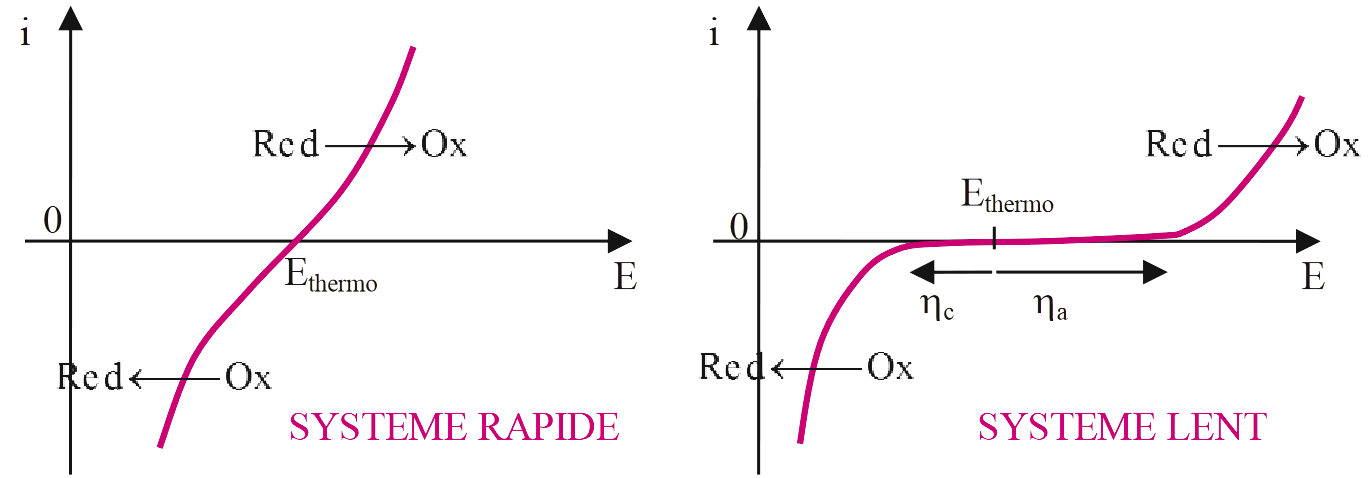
\includegraphics[width=\linewidth]{chimie/i-E/iE-cours.png}
~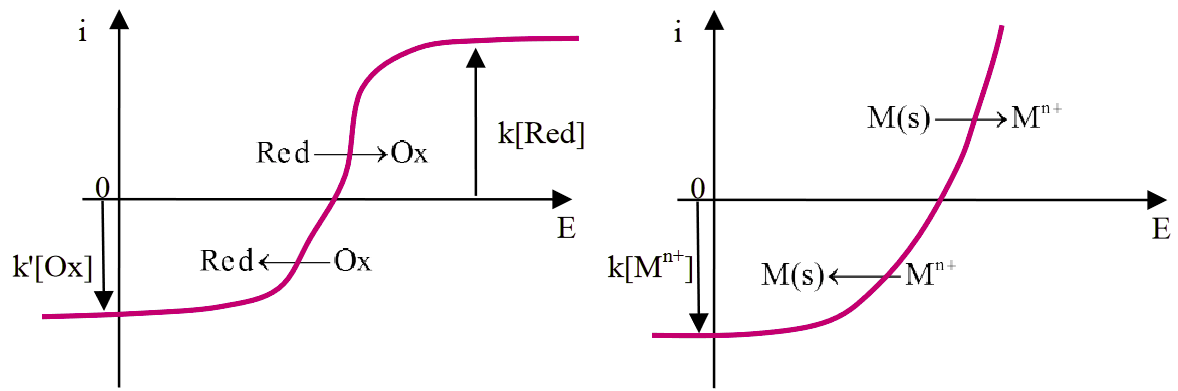
\includegraphics[width=\linewidth]{chimie/i-E/iE-cours2.png}
~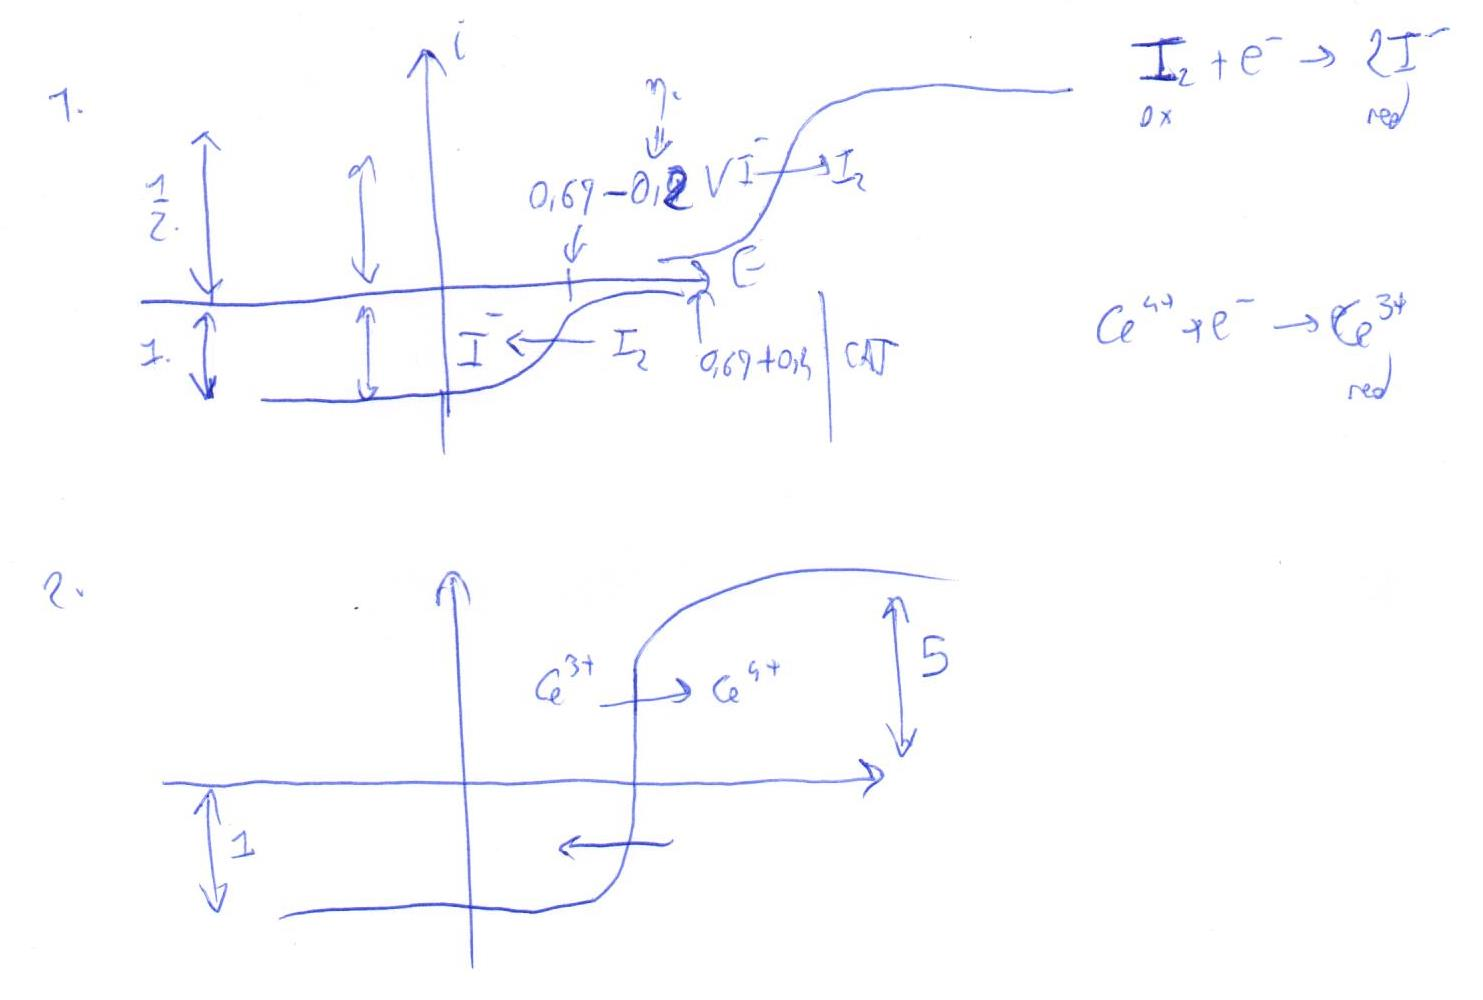
\includegraphics[width=\linewidth]{chimie/i-E/iE-corr.jpg}

\end{solution}

\begin{exercise}{Lecture de courbes $i-E$}{1}{Spé}
{Oxydoréduction, Courbes intensité potentiel}{bermu}

\textsf{Question de cours :} Interpréter quantitativement l’allure des courbes courant-tension suivantes :
\begin{questions}
    \question \hfill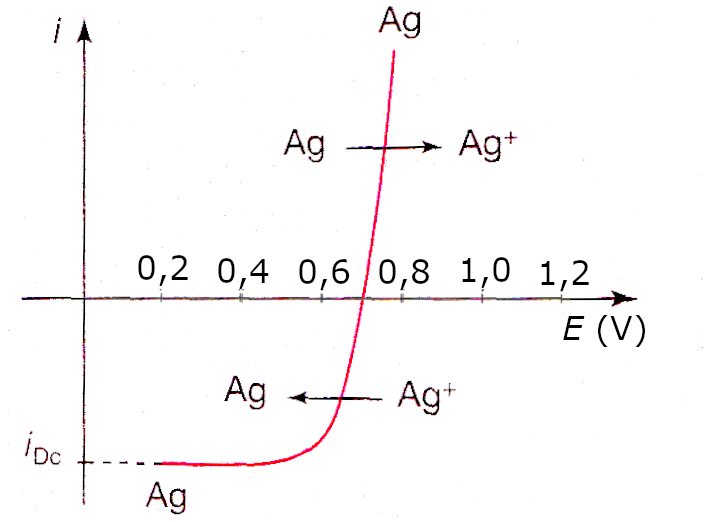
\includegraphics[valign=t,scale=1.5]{chimie/i-E/iE-2.png}\hfill ~
    
    \textsf{Données :} $[\mathrm{Ag^+}] = \SI{1e-2}{mol.L^{-1}}$, $E^\circ\qty\big(\mathrm{Ag^+_{(aq)}/Ag_{(s)}}) = \SI{0.80}{V}$.
    \question \hfill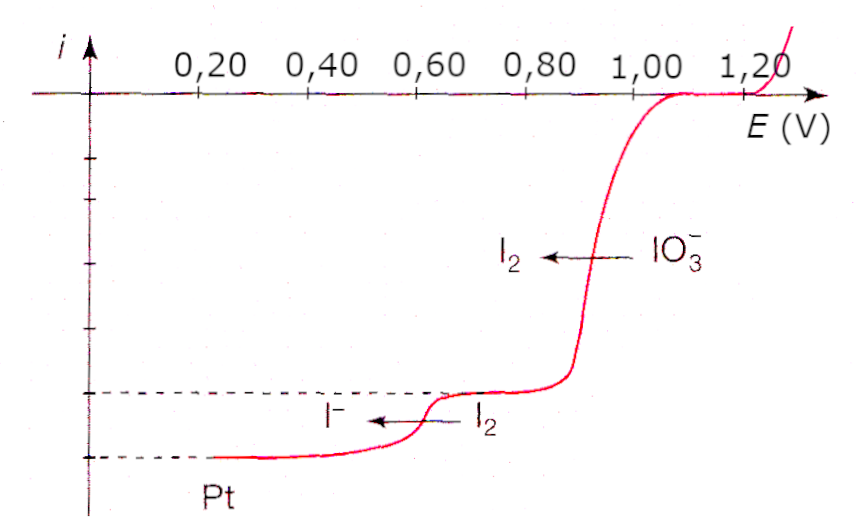
\includegraphics[valign=t,scale=1.5]{chimie/i-E/iE-1.png}\hfill ~

    \textsf{Données :} $E^\circ\qty\big(\mathrm{I_{2,(aq)}/I^-_{(aq)}}) = \SI{0.54}{V}$, $E^\circ\qty\big(\mathrm{IO^-_{3,(aq)}/I_{2,(aq)}}) = \SI{1.19}{V}$.
\end{questions}

\end{exercise}

\begin{solution}

\paragraph{Pistes :}

\begin{questions}
    \question~
        \begin{parts}
            \part Pourquoi n’observe-t-on pas de palier de diffusion anodique pour le système $\mathrm{Ag^+_{(aq)}/Ag_{(s)}}$ ?
            \part Vérifier numériquement la valeur du potentiel à l’équilibre.
            \part Ce système est-il rapide ou lent ?
        \end{parts}
    \question~
        \begin{parts}
            \part Pourquoi observe-t-on des vagues de réduction de hauteur différente ?
            \part Prévoir l’allure de la courbe d’oxydation d’une solution d’iodure sur platine.
        \end{parts}
\end{questions}

\end{solution}
%%%%%%%%%%%%%%%%%%%%%%%%%%%%%%%%%%%%%%%%%%%%%%%%%%%%%%%%%%%%%%%%%%%%%%%%%%%%%%%%%%%%%%%%%%%%%%%%%%%%%%%%%%%%%%

\begin{exercise}{Potentiel mixte}{2}{Spé}
{Oxydoréduction, Courbes intensité potentiel}{bermu}

\begin{questions}
    \questioncours Potentiel mixte.
    \uplevel{Deux électrodes, l’une de fer et l’autre de zinc plongent dans une solution de chlorure de sodium (dont le seul rôle est d’assurer la conduction électrolytique). Elles sont court-circuitées.
    
    On observe un dégagement gazeux au niveau de l’électrode de fer et l’apparition d’un précipité blanc au niveau de l’électrode de zinc.}
    \question Interpréter ces observations à l’aide de courbes intensité-potentiel et évaluer le potentiel mixte de la solution.
\end{questions}

\paragraph{Données}

\begin{itemize}
    \item $E^\circ\qty\big(\mathrm{Fe^{2+}_{(aq)}/Fe_{(s)}}) = \SI{-0.44}{V}$
    \item $E^\circ\qty\big(\mathrm{Zn^{2+}_{(aq)}/Zn_{(s)}}) = \SI{-0.76}{V}$
    \item $\text{p}K_\text{s}(\mathrm{Zn(OH)_{2(s)}/Zr^{2+}_{(aq)}}) = 17.1$
    \item surtension du couple $\mathrm{H^+_{(aq)}/H_{2(g)}}$ sur le fer $\eta = \SI{-0.2}{V}$.
\end{itemize}

\end{exercise}

\begin{solution}

\begin{questions}
    \questioncours $j=0$ ne veut pas dire équilibre thermo !

    \begin{center}
        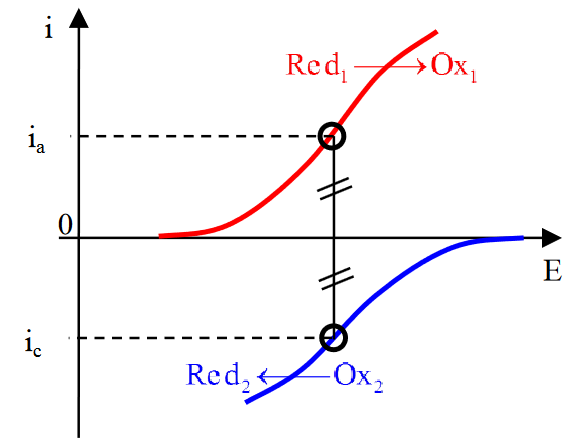
\includegraphics[scale=1.]{chimie/i-E/iE-cours3.png}
    \end{center}
    On observes spontanément un dégagement gazeux au niveau de l’électrode de fer et l’apparition d’un précipité blanc au niveau de l’électrode de zinc.
    \question Dégagement gazeux $=$ H$_2$. $\mathrm{2H^+_{(aq)} + 2 e^- \xrightarrow{Fe_{(s)}} H_{2(g)} }$.
    
    Précipité blanc $= \mathrm{Zn(OH)_{2(s)}}$. $\mathrm{Zn_{s(aq)} + 4 H_2O_{(\ell)} \xrightarrow{Zn_{(s)}} Zn(OH)_{2(s)} + 2H^+_{(aq)} + 2 e^- }$
    
~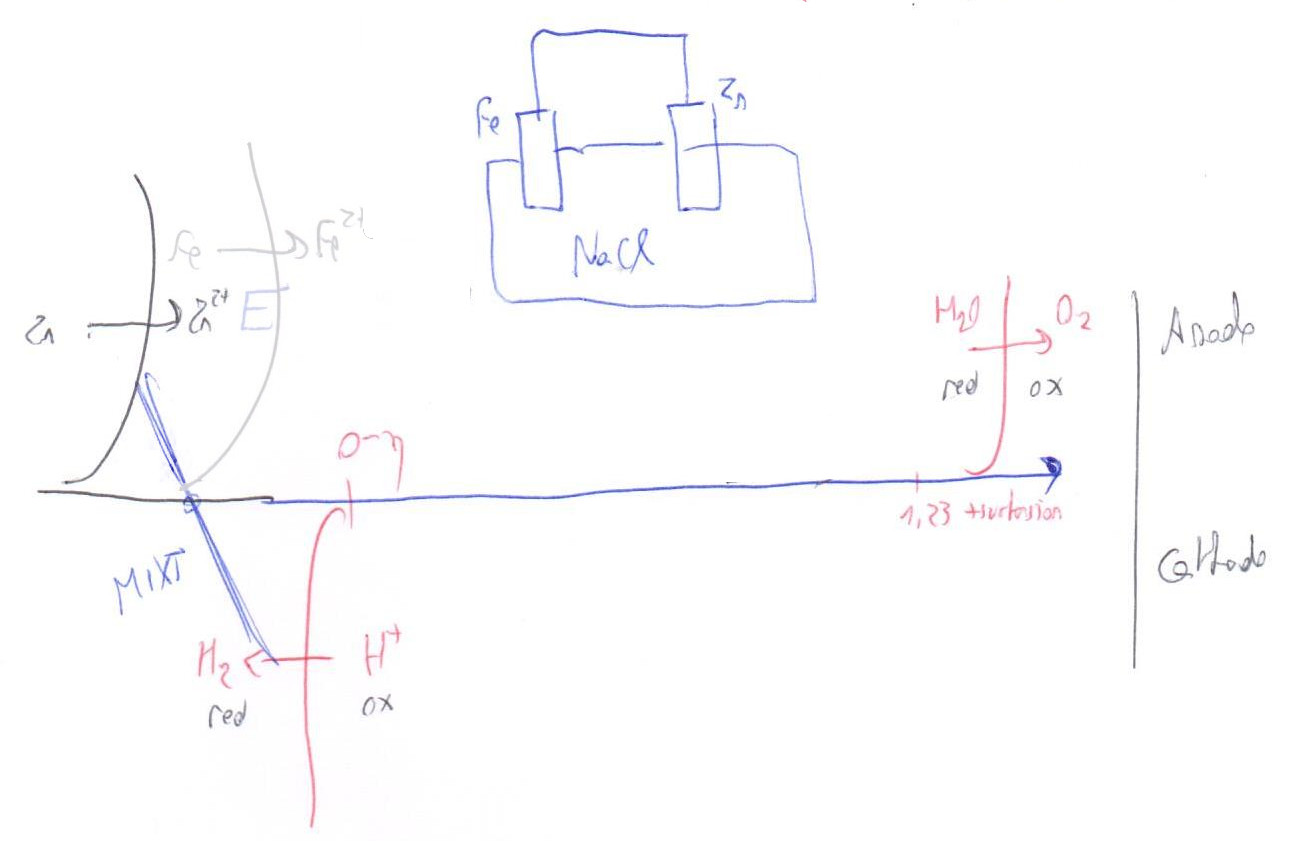
\includegraphics[width=\linewidth]{chimie/i-E/iE-corr2.jpg} 
\end{questions}

\end{solution}

%https://www.lycee-champollion.fr/IMG/pdf/td_no2_chimie_14-15.pdf